\begin{thwbr}
%\chapter[รู้จักกับ Linux]{\makebox[\headwidth][r]{\wayhuge รู้จักกับ \textrm{Linux}}}\label{chap:intro}
\chapter{รู้จักกับลินุกซ์}\label{chap:intro}
\noindent{\fboxsep=12pt \fbox{%
\parbox{.9\headwidth}{\latintext\tt\scriptsize
From: tovalds@klaava.Helsinki.Fi (Linus Benedict Torvalds)\\
To: Newsgroups: comp.os.minix\\
Subject: What would you like to see most in minix?\\
Summary: small poll for my new operating system\\
Message-ID: <1991Aug25.205708.9541@klaava.Helsinki.Fi>\\
\\
Hello everybody out there using minix-I'm doing a (free) operating system (just a hobby, won't be big and professional like gnu) for 386 (486) AT clones. This has been brewing since april, and is starting to get ready. I'd like any feedback on things people like/dislike in minix, as my OS resembles it somewhat (same physical layout of the file-system (due to practical reasons) among otherthings).\\
\\
I've currently ported bash (1.08) and gcc (1.40), and things seems to work. This implies that I'll get something practical within a few months, and I'd like to know what features most people would want. Any suggestions are welcome, but I won't promise I'll implement them:-)\\
\\
\hspace*{\stretch{1}} Linus (torvalds@kruuna.helsinki.fi)\\
\\
PS. Yes-it's free of any minix code, and it has a multi-threaded fs. It is NOT portable (uses 386 task switching etc.), and it probably never will support anything other than AT-harddisks, as that's all I have:-(.
}}
\fboxsep=2pt
%%%% vocab
%\myvocab{Newsgroup : นิวส์กรุป\par Operating System : ระบบปฏิบัติการ\par Linux : ลินุกซ์\par Developer : เดเวลอปเปอร์\par Muti-users : มัลติยูสเซอร์\par Multi-tasks : มัลติทาส์ก\par Personal computer : คอมพิวเตอร์ส่วนบุคคล\par Processor : หน่วยประมวลผล} %
%\begin{center}
%\scalebox{0.65}{\includegraphics{images/news.eps}}\\
%\end{center}
%\vspace{5mm}
\medskip

%
%
เรื่องราวของ{\em ลินุกซ์ (Linux)} เริ่มมาจากข้อความข้างบนที่ส่งถึง Minix \index{general}{minix@Minix}%
\mymemo{คำว่า ``ลินุกซ์'' เป็นศัพท์ที่บัญญัติโดยราชบัณฑิตยสถาน. ชาวต่างชาติบ้างก็อ่านออกเสียงว่า ``ไลนักซ์''. ทางญี่ปุ่นอ่านออกเสียงว่า ``ลินักซ์''.}
\myvocab{m}{Minix}{ระบบปฏิบัติการคล้ายเหมือนยูนิกซ์ที่สร้างขึ้นโดยศาสตราจารย์ Andrew Tanenbaum เพื่อการเรียนการสอนเกี่ยวกับระบบปฏิบัติการ}%
{\em นิวส์กรุป (newsgroup)} เมื่อปี ค.ศ.1991. ข้อความฉบับนี้เขียนโดยนักศึกษาชาวฟินแลนด์ที่มีชื่อว่า Linus Benedict Torvalds\index{general}{linus benedict torvalds@Linus Benedict Torvalds} เพื่อแนะนำ {\em ระบบปฏิบัติการ (Operating System,
OS)} ที่เขาสร้างขึ้น. ใครจะคาดคิดบ้างว่าในเวลาต่อมา, ระบบปฏิบัติการที่เขาสร้างขึ้นที่เรียกว่า {\em Linux} จะเป็นระบบปฏิบัติการที่ใช้กันอย่างแพร่หลายในปัจจุบันและเป็นคู่แข่งที่น่ากลัวของระบบปฏิบัติการอื่นๆ. 

 
\section{{\latintext Linux} คืออะไร?}

``Linux''\index{general}{linux@Linux|see{ลินุกซ์}} หรือที่เรียกในภาษาไทยว่า ``ลินุกซ์'',\index{general}{ลินุกซ์}%
เป็นระบบปฏิบัติการที่สร้างโดยนาย Linux Benedict Torvalds ชาวฟินแลนด์ขณะที่เขาเป็นนักศึกษาอยู่ที่มหาวิทยาลัย Helsinki. หลังจากที่เขาเผยแพร่{\em รหัสต้นฉบับ (source code)} ทางอินเทอร์เน็ตแล้วทำให้มี{\em นักพัฒนาซอฟต์แวร์ (software developer)\index{general}{นักพัฒนาซอฟต์แวร์}} ซึ่งส่วนมากเป็นอาสาสมัครอยู่ทั่วโลกช่วยกันพัฒนาตัวระบบปฏิบัติการเอง, รวมถึงโปรแกรมต่างๆที่ใช้ในระบบด้วย. กล่าวได้ว่าระบบปฏิบัติการลินุกซ์เป็นระบบปฏิบัติการที่เกิดจากอินเทอร์เน็ตและพัฒนาบนอินเทอร์เน็ต.
 
ลินุกซ์เป็นระบบปฏิบัติการแบบ{\em มัลติยูสเซอร์ (multi-users)} %
\myvocab{m}{multi-users}{\emph{มัลติยูสเซอร์}. ความสามารถของระบบปฏิบัติการที่ให้ผู้ใช้หลายคนทำงานได้ในเวลาเดียวกัน}
และ {\em \makebox{มัลติทาส์ก} (multi-tasks)} %
\myvocab{m}{multi-tasks}{\emph{มัลติทาส์ก}. ความสามารถในการแบ่งเวลาการทำงานของหน่วยประมวลผลเมื่อมีงานหลายอย่างที่ต้องทำ. เป็นผลให้ดูเหมือนว่าหน่วยประมวลผลข้อมูลสามารถทำงานหลายอย่างได้ในเวลาเดียวกัน.}%
ที่ใช้ได้กับระบบคอมพิวเตอร์หลายประเภท. ระบบคอมพิวเตอร์ที่ลินุกซ์ใช้กันอย่างแพร่หลายได้แก่ระบบ{\em คอมพิวเตอร์ส่วนบุคคล (Personal Computer, PC)} ที่ใช้{\em หน่วยประมวลผล (Processor)} ที่มา{\em สถาปัตยกรรม (architechture)} แบบ CISC (Complex Instruction Set Computer) เช่นหน่วยประมวลผลตระกูล Intel, AMD เป็นต้น. ลินุกซ์ยังสามารถใช้งานกับระบบคอมพิวเตอร์ที่ใช้หน่วยประมวลผลอื่นๆได้ด้วยเช่น MIPS, SPARC, PowerPC ฯลฯ, โดยแก้ไขรหัสต้นฉบับของลินุกซ์บางส่วน.

%%% myvocab
%\myvocab{Source code : รหัสต้นฉบับ\par UNIX : ยูนิกซ์\par Compatibility : ความเข้ากันได้\par Compile : คอมไพล์\par Execute : กระทำการ\par Kernel : เคอร์เนล\par Process : โปรเซส\par Memory : หน่วยความจำ\par Device : ดีไวส์\par Hard disk : ฮาร์ดดิกส์\par X window system : ระบบ X วินโดว์\par Desktop environemtn : ระบบเดกส์ท็อป\par Complier : คอมไพเลอร์\par Interpreter : อินเทอร์พรีเตอร์\par Editor : บรรณาธิกรณ์\par License : ใบอนุญาต\par copying : การทำสำเนา\par distubution : การแจกจ่าย\par modification : การแก้ไข\par Download : ดาว์นโหลด} %
ลินุกซ์เป็นระบบปฏิบัติการที่คล้ายเหมือนกับระบบปฏิบัติการ{\em ยูนิกซ์ (UNIX)}. กล่าวคือ, ลินุกซ์ออกแบบโดยใช้{\em แนวความคิด (concept)} ของระบบปฏิบัติการยูนิกซ์เป็นต้นแบบ. แต่ลินุกซ์เริ่มสร้างขึ้นโดยนาย Linus Torvalds เพียงลำพังโดยไม่ได้ลอกเลียนหรือสืบทอดรหัสต้นฉบับจากยูนิกซ์แต่อย่างใด.
ลินุกซ์ถูกสร้างขึ้นมาให้ทำงานทุกอย่างที่ระบบปฏิบัติการยูนิกซ์ทำได้โดยยึดมาตรฐาน {\em
POSIX (Portable Operating System Interface based on UNIX)}.\index{general}{posix@POSIX} %
\myvocab{p}{POSIX}{ข้อกำหนดมาตรฐานว่าระบบปฏิบัติการที่สามารถใช้งานได้กับฮาร์ดแวร์ต่างระบบนั้นต้องมีรายละเอียดคุณสมบัติอย่างไร. มาตรฐานนี้กำหนดโดยองค์กร The Institute
of Electrical and Electronic Engineers (IEEE).}
%
ซึ่งหมายความว่าโปรแกรมที่ใช้บนลินุกซ์มี{\em ความเข้ากันได้ (compatibility)}\index{general}{compatibility} กับระบบปฏิบัติการยูนิกซ์อื่นๆในระดับรหัสต้นแบบ. กล่าวคือสามารถนำรหัสต้นฉบับของโปรแกรมที่ใช้ในลินุกซ์ไป{\em คอมไพล์ (compile)}\index{general}{compile} บนระบบปฏิบัติการยูนิกซ์อื่นๆและ{\em กระทำการ (execute)} ได้โดยไม่ต้องแก้ไขรหัสต้นฉบับหรือแก้ไขเพียงเล็กน้อยเท่านั้น.\mymemo{การที่นำรหัสต้นฉบับของโปรแกรมบนระบบหนึ่งไปแก้ไขและคอมไพล์บนระบบอื่นเรียกว่าการ porting. โปรแกรมที่มีคุณสมบัตินี้เรียกได้ว่า portable หรือมีความสามารถในการ port (portability).} ในทางกลับกัน, ผู้ใช้สามารถนำรหัสต้นฉบับของโปรแกรมที่ใช้ในระบบปฏิบัติการยูนิกซ์อื่นๆมาคอมไพล์แล้วกระทำการบนระบบปฏิบัติการลินุกซ์ได้เช่นเดียวกัน. 

%\label{aa}
%\ifodd\pageref{aa} \parbox{\headwidth}{\rule{\headwidth}{1pt}}
%\else
%\noindent\parbox{\headwidth}{\leftskip=\moveback \rule{\headwidth}{1pt}}
%\fi
%\label{check1}\ifthenelse{\isodd{\pageref{check1}}}{XXXXX}{YYYYY}



เมื่อกล่าวถึงคำว่า ``ลินุกซ์'' เดี่ยวๆ, เราสามารถตีความได้หลายความหมาย. ในความหมายเฉพาะเรื่อง, ลินุกซ์หมายถึงแก่นของระบบปฏิบัติการที่เรียกว่า{\em เคอร์เนล (kernel)}\index{general}{kernel} หรือเรียกให้ชัดเจนว่า {\em ลินุกซ์เคอร์เนล (linux kernel)} ซึ่งเป็นโปรแกรมพิเศษ, 
ทำหน้าแบ่งเวลาทำงานของหน่วยประมวลผลให้{\em โปรเซส (process)} ต่างๆ, จัดการการใช้{\em หน่วยความจำ (memory)}, 
ควบคุมการทำงานของ{\em ดีไวส์ (device)} ไม่ว่าจะเป็น{\em ฮาร์ดดิกส์ (hard disk)}, {\em I/O Port} ฯลฯ.
ในความหมายโดยรวมหรือความหมายทั่วไป, ลินุกซ์หมายถึง {\em Operating Enviroment}\index{general}{open operating environment@Operating Environment} ซึ่งหมายถึงเคอร์เนลและกลุ่มของซอฟต์แวร์ต่างที่นำมารวมกันให้เป็นระบบ.
ตัวอย่างโปรแกรมต่างๆที่ใช้กับระบบปฏิบัติการลินุกซ์ได้แก่ {\em ระบบ X วินโดว์  (X window system)}, {\em ระบบเดกส์ท็อป (desktop environment)}, {\em คอมไพเลอร์ (compiler)}, {\em อินเทอร์พรีเตอร์ (interpreter)}, {\em บรรณาธิกรณ์ (editor)} เป็นต้น. สำหรับบุคคลทั่วไปถ้าพูดถึง ``ลินุกซ์'' จะหมายถึง Operating Environment แต่สำหรับนักพัฒนาซอฟต์แวร์หรือโปรแกรมเมอร์, ``ลินุกซ์'' อาจจะมีความหมายลึกกว่านั้นซึ่งเจาะจงถึงเคอร์เนล.

\section{ประวัติความเป็นมาของลินุกซ์}

%\begin{wrapfigure}{l}{56mm}
%\center
%\scalebox{0.7}{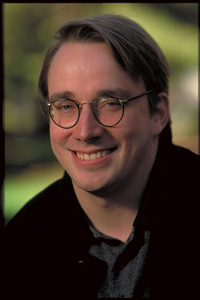
\includegraphics{images/linus.eps}}
%\caption{Linus Benedict Torvalds}
%\end{wrapfigure}
ระบบปฏิบัติการลินุกซ์เริ่มสร้างในปี ค.ศ.  1991
โดยนักศึกษามหาวิทยาลัยชาวฟินแลนด์ที่ชื่อ 
 Linus Torvalds \cite{JustForFun}.  Linus\index{general}{linus benedict torvalds@Linus Benedict Torvalds!Linux Torvalds}
เป็นคนที่สนใจและคลุกคลีกับคอมพิวเตอร์มาตั้งแต่เด็ก. เมื่อเขาเป็นนักศึกษาปีหนึ่งที่มหาวิทยาลัย
Helsinki, เขาได้รู้จักกับระบบปฏิบัติการยูนิกซ์ซึ่งแตกต่างจากระบบปฏิบัติการที่ใช้กับคอมพิวเตอร์ส่วนบุคคล. 
การที่เขาได้รู้จักกับยูนิกซ์นี้เองเป็นจุดเริ่มต้นทำให้เขาสนใจศึกษาการทำงานของระบบปฏิบัติการ.

หนังสือ \emph{Operating Systems: Design and
Implementation} เป็นหนังสือที่เขาอ่านประกอบการเรียนเกี่ยวกับเรื่องระบบปฏิบัติการ. หนังสือเล่มนี้เขียนโดย Andrew Tanenbaum\index{general}{andrew tanenbaum@Andrew Tanenbaum} ซึ่งเป็นอาจารย์มหาวิทยาลัยในประเทศเนเธอร์แลนด์.  Andrew Tanenbaum
นอกจากจะเขียนหนังสือเกี่ยวกับระบบปฏิบัติการแล้วเขายังสร้างระบบปฏิบัติการขนาดเล็กคล้ายยูนิกซ์ที่มีชื่อว่า {\em มินิกซ์ (Minix)\index{general}{minix@Minix}} สำหรับการเรียนการสอนระบบปฏิบัติการอีกด้วย. 
หนังสือเล่มนี้เป็นแรงบันดาลใจและเป็นชนวนความคิดให้ Linus
สร้างระบบปฏิบัติการด้วยตัวเอง.  

ในปี 1991, Linux ซื้อคอมพิวเตอร์ส่วนบุคคลมาใช้งาน. คอมพิวเตอร์ที่เขาซื้อเป็นคอมพิวเตอร์ส่วนบุคคลที่ใช้หน่วยประมวลผลของ Intel รุ่น 80386 และระบบปฏิบัติการที่มาพร้อมกับเครื่องคอมพิวเตอร์นั้นได้แก่ MS DOS. นอกจากนั้นเขาสั่งซื้อระบบปฏิบัติการมินิกซ์ต่างหากเพื่อมาติดตั้ง% 
%\glossindex{install}{การนำโปรแกรมหรือ OS บรรจุในหน่วยความจำถาวรเช่น
%harddisk เพื่อใช้งาน.} 
ในคอมพิวเตอร์เครื่องใหม่ของเขาแทน MS DOS สำหรับศึกษาการทำงานของระบบปฏิบัติการ. เพราะว่ามินิกซ์เป็นระบบปฏิบัติเพื่อการศึกษาไม่ใช่เพื่อการใช้งาน, ระบบบางอย่างในมินิกซ์ใช้งานได้ไม่ดีนักและสิ่งที่เขาไม่ชอบคือ{\em เทอร์มินอลเอมูเลเตอร์ (terminal emulator) }ของมินิกซ์. เขาจึงตัดสินใจเริ่มสร้างโปรแกรมเทอร์มินอลเอมูเลเตอร์%
\myvocab{t}{terminal emulator}{\emph{เทอร์มินอลเอมูเลเตอร์}. โปรแกรมที่ใช้ในการแสดงผลในรูปของตัวอักษรผ่านทางหน้าจอโดยการป้อนข้อมูลเข้าผ่านทางคีย์บอร์ด}%
ด้วย{\em ภาษาแอสเซมบลี (assembly language)} เอง.

เพื่อที่จะอ่านนิวส์กรุปของมหาวิทยาลัยผ่าน{\em โมเด็ม (Modem)} จากที่บ้าน, เขาต้องสร้างเทอร์มินัลเอมูเลเตอร์ที่ทำงาน 2 อย่างพร้อมๆกันคือ อ่านข้อมูลจากโมเด็มแล้วแสดงผลทางหน้าจอ,
และรับข้อมูลจากคีย์บอร์ดแล้วส่งต่อให้โมเด็ม.
การทำงานสองอย่างในเวลาเดียวกันใช้หลักการที่เรียกว่า {\em task switching}\index{general}{task switching} ซึ่งเป็นพื้นฐานของระบบปฏิบัติการ.
โปรแกรมเทอร์มินอลเอมูเลเตอร์ที่เขาสร้างเก็บบันทึกอยู่ในแผ่น{\em ฟล็อปปี้ดิกส์ (floppy disk)}
เพราะฉะนั้นเวลาที่เขาจะใช้โปรแกรมต้อง{\em บูต (boot)} โปรแกรมจากแผ่นฟล็อปปี้ดิกส์โดยตรง. ปัญหาที่ต้องแก้มีมากขึ้นเมื่อเขาต้องการดาวน์โหลดไฟล์ผ่านทางโมเด็มเก็บบันทึกลงฮาร์ดดิกส์. ปัญหานี้ทำให้เขาต้องศึกษาเกี่ยวกับ {\em file system} และเขาไม่ท้อถอย. Linus
เขียน{\em ไดร์เวอร์ (driver)} ของฮาร์ดดิกส์และทำให้เทอร์มินอลเอมูเลเตอร์เก็บข้อมูลลงฮาร์ดดิกส์จนได้. ในที่สุดเทอร์มินอลเอมูเลเตอร์ที่เป็นโปรแกรมเล็กๆ, เดิมเขียนขึ้นเพื่ออ่านนิวส์กรุปก็เริ่มเปลี่ยนเป็นระบบปฏิบัติการทีละเล็กละน้อย. 

ระบบปฏิบัติการเริ่มเป็นรูปเป็นร่างชัดเจนเมื่อ Linus ทำการ{\em พอร์ต (port)}\index{general}{port (กริยา)} %
\myvocab{p}{port}{\emph{พอร์ต}(กริยา). การดัดแปลงต้นฉบับโปรแกรม, คอมไพล์ให้ใช้บนระบบปฏิบัติการที่แตกต่างกันหรือสถาปัตยกรรมคอมพิวเตอร์ที่แตกต่างกันได้}\myvocab{x}{X window system}{\emph{X วินโดว์}. ระบบการแสดงผลกราฟฟิกส์ผ่านทางจอภาพในรูปแบบของหน้าต่างหลายบาน. เป็นโครงการของ MIT ที่พัฒนาต่อมาจาก W windows system ของ Stanford. ระบบ X วินโดว์ที่ใช้ในลินุกซ์เป็นโครงการของ Xfree86 ซึ่งพัฒนา X เซิฟร์เวอร์สำหรับวีดีโอการ์ดต่างๆ. สังเกตุว่าเขียนว่า X window ไม่ใช่ X windows.}
{\em เชลล์ (shell)} 
ซึ่งเป็นตัวโปรแกรมรับคำสั่งจากคีย์บอร์ดส่งต่อให้ระบบปฏิบัติการ. ระบบปฏิบัติเริ่มสมบูรณ์เมื่อเขาพอร์ต{\em คอมไพเลอร์ภาษา  C (C compiler)} สำเร็จ.
นั่นหมายความว่าเขาสามารถนำรหัสต้นฉบับของโปรแกรมอื่นมาคอมไพล์และใช้ได้กับระบบปฏิบัติการที่เขาสร้างไว้. ความต้องการ, ความพยายาม, และการไม่ยอมแพ้ของนาย Linus นี่เองที่ทำให้เกิดระบบปฏิบัติการที่เรียกว่า ``ลินุกซ์'' ในวันนี้.

หลังจากที่  Linus เปิดเผยระบบปฏิบัติการที่เขาสร้างผ่านทางอินเทอร์เน็ต. นักพัฒนาซอฟต์แวร์จากทั่วโลกที่สนใจเริ่มพอร์ตโปรแกรมต่างๆที่ใช้ในยูนิกซ์ให้ใช้ได้กับลินุกซ์เช่น {\em ระบบ X วินโดว์ (X window system)}%
, ยูทิลิตี้โปรแกรมต่างๆที่จาก  Free Software Foundation (GNU)
และอื่นๆ. นอกจากการพอร์ตโปรแกรมที่มีอยู่แล้ว, โปรแกรมบางอย่างสร้างขึ้นสำหรับใช้บน
ลินุกซ์ปัจจุบันพอร์ตไปใช้ในระบบปฏิบัติการยูนิกซ์ด้วยเช่น {\em GNOME} เป็นต้น. สิ่งที่สำคัญอีกอย่างคือการพอร์ตตัวระบบปฏิบัติการลินุกซ์เองให้ใช้ได้กับ{\em สถาปัตยกรรมคอมพิวเตอร์ (computer architecture)} อื่นๆ เช่น  Atari, Alpha, SPARC เป็นต้น.



% สิทธิบัตร (patent), ลิขสิทธิ์ (copyright), ใบอนุญาต (license)
%\section{ใบอนุญาตและสิทธิ์ในการใช้ซอฟต์แวร์}
\section{กฏหมายกับซอฟต์แวร์}
\mymemo{เนื่องจากผู้เขียนไม่ใช่ผู้เชี่ยวชาญด้านกฏหมาย, เนื้อหาที่เกี่ยวกับลิขสิทธิ์, ใบอนุญาต และสิทธิบัตรที่แนะนำนี้อาจจะไม่ใช่ข้อมูลที่เที่ยงตรง. สำหรับผู้ที่สนใจกรุณาหาหนังสือหรือเว็บไซด์ \cite{thaiip} ที่เกี่ยวกับกฏหมายอ่านประกอบ.}หนังสือเล่มนี้เป็นหนังสือเกี่ยวกับลินุกซ์ไม่ใช่หนังสือที่เกี่ยวกับกฏหมาย. แต่หลีกเลี่ยงไม่ได้ที่จะต้องกล่าวถึงเพราะซอฟต์แวร์ไม่ว่าจะเป็นลินุกซ์เคอร์เนลหรือโปรแกรมต่างๆที่ผู้ใช้ใช้อยู่ถึงแม้ว่าจะ ``ฟรี'' แต่ไม่ได้หมายความว่าเราจะทำอะไรก็ได้กับซอฟต์แวร์เหล่านั้น.

\subsection{ลิขสิทธิ์}
{\em ลิขสิทธิ์ (copyright)} \index{general}{ลิขสิทธิ์}\index{general}{copyright|see{ลิขสิทธิ์}} คือสิทธิ์ที่ผู้สร้างสรรค์พึงจะได้จากผลงานที่สร้าง. ผลงานในที่นี้ได้แก่ ซอฟต์แวร์, หนังสือ, ภาพยนต์, เพลง เป็นต้น. ผู้ถือสิทธิ์มีสิทธิ์ในผลงานของตัวเองเช่น สิทธิ์ในการขาย, สิทธิ์ห้ามทำสำเนา, สิทธิ์ในการแจกจ่าย ฯลฯ. ซอฟต์แวร์ลิขสิทธิ์คือซอฟต์แวร์ที่ได้รับการคุ้มครองโดยกฎหมายลิขสิทธิ์. การที่ผู้อื่นที่ไม่ใช่เจ้าของผลงานนั้นๆจะใช้ต้องได้รับอนุญาตจากผู้ถือสิทธิ์ก่อนที่จะใช้ผลงานนั้น. ซอฟต์แวร์ที่ไม่มีลิขสิทธิ์ได้แก่ซอฟต์แวร์ที่ไม่มีการคุ้มครองใดๆทางกฏหมาย เช่นซอฟต์แวร์ที่ประกาศเป็น{\em สาธารณะสมบัติ (public domain)}\index{general}{สาธารณะสมบัติ}\index{general}{public domain|see{สาธารณะสมบัติ}}.

ตัวอย่างซอฟต์แวร์เช่นลินุกซ์เคอร์เนลเป็นซอฟต์แวร์ที่มีลิขสิทธิ์และผู้ที่ถือครองลิขสิทธิ์ได้แก่นาย Linus Torvalds ซึ่งเป็นผู้สร้าง. ตามหลักแล้วไม่ว่าจะเป็นใครก็ตามที่ต้องการใช้ลินุกซ์ต้องได้รับอนุญาตจากนาย Linus ก่อนจึงจะใช้ได้. แต่ในความเป็นจริงผู้ใช้สามารถใช้ลินุกซ์ได้โดยไม่ต้องขออนุญาตเพราะนาย Linus ได้ให้อนุญาตแล้วโดยใช้{\em ใบอนุญาต (license)} ที่เรียกว่า GNU General Public License ต่อลินุกซ์เคอร์เนลที่เขาสร้างขึ้น.

\subsection{ใบอนุญาต}
ตั้งแต่เริ่มต้นเรื่องราวของคอมพิวเตอร์, ซอฟต์แวร์คือสินค้าแต่เป็นสินค้าที่ต่างจากสินค้าทั่วไปตรงที่ซอฟต์แวร์เป็นสินค้าเชิงนามธรรมมากกว่ารูปธรรม. ตามธรรมชาติของซอฟต์แวร์, ซอฟต์แวร์เป็นข้อมูลที่เก็บอยู่ในสื่อกลางต่างๆได้. สามารถทำสำเนาส่งต่อให้คนอื่นได้. ใช้ได้กับคอมพิวเตอร์ไม่เจาะจงว่าต้องเป็นเครื่องใดๆ. ธรรมชาติของซอฟต์แวร์นี้เองเป็นปัญหาสำหรับผู้ผลิตซอฟต์แวร์เชิงพาณิชย์. กล่าวคือถ้าผู้ผลิตซอฟต์แวร์ไม่ทำสัญญากับผู้ที่ได้ซอฟต์แวร์, ผู้ที่ได้ซอฟต์แวร์นั้นสามารถทำสำเนาแจกจ่าย, หรือใช้กับคอมพิวเตอร์ได้ไม่เลือก. เป็นผลให้ผู้ผลิตซอฟต์แวร์ไม่สามารถดำเนินธุรกิจด้วยการขายซอฟต์แวร์ได้. นี่เองเป็นที่มาของ{\em ใบอนุญาต (license)}.\index{general}{license|see{ใบอนุญาต}}\index{general}{ใบอนุญาต}

โดยปรกติแล้วซอฟต์แวร์จะมีใบอนุญาตในการใช้งานกำกับมาด้วย. ใบอนุญาตได้แก่ข้อตกลงระหว่างผู้สร้าง, เจ้าของ, หรือผู้จำหน่ายซอฟต์แวร์กับผู้ที่ได้รับซอฟต์แวร์นั้นๆซึ่งเนื้อหาของข้อตกลงจะแตกต่างกันออกไปตามกรณี. โดยปรกติ, ในอนุญาตจะจำกัดสิทธิ์ต่างๆที่พึงกระทำได้กับซอฟต์แวร์เช่นห้ามทำสำเนาแจก, ห้ามติดตั้งซอฟต์แวร์ลงในเครื่องคอมพิวเตอร์เกินหนึ่งเครื่องเป็นต้น. แน่นอนว่าในทางปฏิบัติ, ผู้ที่ได้ซอฟต์แวร์นั้นมาสามารถกระทำสิ่งเหล่านี้ได้แต่จะเป็นการละเมิดข้อตกลงและถือว่ามีความผิด, อาจถูกดำเนินคดีตามกฏหมายต่อไป.


\subsubsection{GNU General Public License}\index{general}{gnu general public license@GNU General Public License}

ลินุกซ์เคอร์เนลให้อิสระแก่ผู้ใช้ครอบคลุมเรื่องการทำสำเนา (copying), การแจกจ่าย (distribution) และการแก้ไข (modification). ใบอนุญาตที่ลินุกซ์เลือกใช้ได้แก่ {\em GNU General Public License (GNU GPL)}. ใบอนุญาตแบบ GPL\index{general}{gpl@GPL|see{GNU General Publice License}} นี้สร้างขึ้นโดยองค์กรที่เรียกว่า {\em Free Software Foundation}\index{general}{free software foundation@Free Software Foundation}\index{general}{gnu@GNU} 
%%%
%\marginpar{\includegraphics{gnu-head-sm.eps}}
\mymemo{Free Software Foundation เป็นองค์กรอิสระไม่หวังผลกำไรซึ่งก่อตั้งโดย Richard Stallman
เมื่อปี{ค.ศ.} 1982. จุดประสงค์ขององค์กรนี้คือสร้างระบบยูนิกซ์ที่เสรี. ซอฟต์แวร์ที่มีชื่อเสียงที่พัฒนาโดยองค์กรนี้ได้แก่ GNU C compiler,
GNU Emacs ฯลฯ. 

Free Software Foundation มีชื่อเรียกทั่วไปว่า GNU เป็นคำย่อแบบ recursive ของคำว่า ``{\bf G}NU is {\bf N}ot {\bf U}nix''}
%%%
ก่อตั้งและดำเนินการโดยนาย Richard Stallman\index{general}{richard stallman@Richard Stallman}. 

ใบอนุญาตแบบ GPL นี้เองที่ทำให้ลินุกซ์ต่างจากระบบปฏิบัติการทั่วๆไป. โดยปรกติแล้วระบบปฏิบัติการจะพัฒนาโดยองค์กรหรือบริษัทในกลุ่มเล็กๆ. ไม่มีการเปิดเผยรหัสต้นฉบับแก่สาธารณะ, ผู้ใช้ไม่สามารถทำสำเนาหรือแจกจ่ายให้คนอื่นต่อได้. ระบบปฏิบัติการลินุกซ์มีความคิดที่แตกต่างกับสิ่งที่กล่าวมาอย่างสิ้นเชิง. ลินุกซ์เป็นระบบปฏิบัติการที่ฟรี. ผู้ที่ต้องการใช้ลินุกซ์ไม่มีความจำเป็นที่ต้องเสียเงินซื้อ, สามารถ{\em ดาวน์โหลด (download)}
จากอินเทอร์เน็ต \cite{kernel}. และผู้ใช้มีสิทธิ์ที่จะแจกจ่ายต่อไปได้โดยไม่ผิดกฎหมายตราบที่ผู้ใช้ยังปฏิบัติตามใบอนุญาต GPL ระบุไว้. คำว่า ``ฟรี'' ในที่นี้ไม่ได้หมายความว่าราคาเป็น ``ศูนย์'' แต่หมายถึงความเป็น ``อิสระเสรี'' ที่ผู้ใช้กระทำได้. การที่ลินุกซ์ใช้ใบอนุญาตแบบ GPL มีผลดีคือให้อิสระเสรีแก่ผู้ใช้. เปิดโอกาสให้นักพัฒนาซอฟต์แวร์สามารถศึกษารหัสต้นฉบับ, และพัฒนาปรับปรุงแก้ไขโปรแกรมต่อไปให้ดียิ่งขึ้น. GPL ยังระบุถึง{\em งานสืบทอด (derived work)} ของซอฟต์แวร์ที่มีใบอนุญาตเป็นแบบ GPL ด้วยว่างานสืบทอดจะใช้ใบอนุญาตแบบ GPL โดยปริยาย. กล่าวคือถ้าเป็นงานที่สืบทอดมาจากงาน GPL งานนั้นต้องเป็น GPL ด้วย. บุคคลใดๆมีอิสระทำสำเนา, แจกจ่าย, แก้ไขรหัสต้นฉบับของงานสืบทอดได้. เราสามารถกล่าวได้ว่าเหตุที่ลินุกซ์ใช้กันอย่างแพร่หลายและมีการแก้ไขปรับปรุงให้ทันสมัยทันเหตุการณ์เป็นผลของการที่ลินุกซ์ใช้ใบอนุญาต GPL นี่เอง.

\subsubsection{GNU Lesser General Public License}\mymemo{เดิมคือใบอนุญาต GNU Library General Public License.}
สำหรับงานสืบทอดที่ทำต่อหรือใช้รหัสต้นฉบับของซอฟต์แวร์ที่มีใบอนุญาตแบบ GPL, ตัวใบอนุญาตระบุไว้ว่างานสืบทอดจะต้องใช้ใบอนุญาตแบบ GPL ไปโดยปริยาย \cite{gpl}. หมายความว่าโปรแกรมเชิงพาณิชย์ที่สืบทอดหรือใช้รหัสต้นฉบับจากซอฟต์แวร์ที่มีใบอนุญาตแบบ GPL ต้องมีใบอนุญาตเป็นแบบ GPL ไปด้วย. ในกรณีอาจเป็นผลเสียในเชิงพาณิชย์เพราะซอฟต์แวร์ที่ผลิตออกมาจะกลายเป็นซอฟต์แวร์ที่สามารถทำสำเนา, แจกจ่ายได้, ขอรหัสต้นฉบับได้ไปโดยปริยาย. เหตุนี้เองทาง FSF จึงออกในอนุญาตที่เรียกว่า {\em GNU Lesser General Public License (LGPL)} ที่ลดหย่นสิทธิ์ของผู้ใช้เล็กน้อยตรงที่เปิดโอกาสให้ซอฟต์แวร์เชิงพาณิชย์สามารถใช้รหัสต้นฉบับของซอฟต์แวร์ซึ่งรวมไปถึง{\em ไลบรารี (library)} ที่มีใบอนุญาตแบบ GPL ได้โดยที่งานสืบทอดนั้นยังคงใช้ใบอนุญาตของตัวเองที่ไม่ใช่ GPL ก็ได้.

สรุปได้ว่า LGPL ให้อิสระต่อผู้ใช้น้อยลง (lesser) เมื่อเทียบกับใบอนุญาตแบบ GPL. ในทางตรงกันข้ามเป็นการเปิดโอการให้ซอฟต์แวร์เชิงพาณิชย์ที่ถือเป็นงานสืบทอดใช้ซอฟต์แวร์หรือไลบรารีที่มีใบอนุญาตเป็น GPL ได้โดยยังคงใบอนุญาตของตัวเอง. 

การตีความงานสืบทอดว่าคืออะไรยังไม่ค่อยกระจ่างมากนัก, คงต้องยกเป็นเรื่องของกฏหมาย. ตัวอย่างงานสืบทอดที่ชัดเจนได้แก่การแก้ไข, เพิ่มเติม, ปรับแต่งงานที่เป็นแบบ GPL ถือว่าเป็นงานสืบทอดอย่างเห็นได้ชัด. ซอฟต์แวร์ที่ใช้ไลบรารีที่ไม่ได้สร้างเองก็ถือว่าเป็นงานสืบทอดเช่นกัน. ดังนั้นไลบรารีที่เป็นมาตรฐานและใช้กันมากของ FSF มันจะใช้ใบอนุญาตแบบ LGPL เช่นไลบรารี C ของ GNU เป็นต้น.\mymemo{การคอมไพล์โปรแกรมเช่นโปรแกรมที่เขียนด้วยภาษา C จะใช้ไลบรารี C โดยปริยาย. แต่เนื่องจากไลบรารี C ของ GNU มีใบอนุญาตเป็น LGPL เพราะฉะนั้นโปรแกรมที่ใช้ไลบรารีนี้ไม่จำเป็นต้องเป็น GPL ก็ได้.}



%\mymarginpar{\scalebox{0.6}{\includegraphics{images/gnu-head-sm.eps}} }. 
%%% myvocab
%\myvocab{Free software : ซอฟต์แวร์เสรี\par Run : กระทำการ, รัน\par Copy : ทำสำเนา, ก็อปปี้\par Distribute : แจกจ่าย}
\subsubsection{ใบอนุญาตแบบอื่นๆ}

ในขณะที่ลินุกซ์เคอร์เนลใช้ใบอนุญาตแบบ GPL, โปรแกรมต่างๆที่นำมารวมเข้าเป็นระบบใช้งานไม่จำเป็นต้องใช้ใบอนุญาตแบบ GPL ก็ได้. โปรแกรมที่ใช้กับลินุกซ์เคอร์อาจจะใช้ใบอนุญาตแบบอื่นๆ \cite{license} ตามตัวอย่างที่แสดงในตารางที่ \ref{tab:license}.

\begin{table}
\center
\caption{ตัวอย่างประเภทของใบอนุญาตต่างๆแบ่งตามความเสรี}
\medskip
\label{tab:license}
\begin{tabular}{p{.4\linewidth}p{.5\linewidth}}
\hline
\multicolumn{1}{c}{ประเภทของใบอนุญาต} &  \multicolumn{1}{c}{ตัวอย่าง}\\
\hline
GPL-Compatible Free Software Licenses & GPL, LGPL, Public Domain, X11 License, BSD (modified)\\
GPL-Incompatible, Free Software Licenses & BSD (original), Open Software License, Apache License, Mozilla Public License (MPL), Q Public License (QPL), PHP License\\
Non-Free Software Licenses & Open Public License, Aladdin Free Public License, Microsoft's Shared Source License\\
\hline
\end{tabular}
\end{table}

\subsection{สิทธิบัตร}
{\em สิทธิบัตร (patent)}\index{general}{สิทธิบัตร}\index{general}{patent|see{สิทธิบัตร}} คือหนังสือสำคัญที่ออกให้เพื่อคุ้มครองการประดิษฐ์ หรือการออกแบบผลิตภัณฑ์. การประดิษฐ์นี้รวมถึงกรรมวิธีซึ่งได้แก่ขั้นตอนวิธี (algorithm) ด้วย. หมายความว่าถ้ามีใครไปจดสิทธิบัตรขั้นตอนวิธีใดๆก่อนแล้วผู้พัฒนาซอฟต์แวร์ใช้ขั้นตอนเดียวกันในการสร้างซอฟต์แวร์ไม่ว่าจะคิดเองหรือไม่ต้องขออนุญาตหรือจ่ายค่าตอบแทนกับผู้ที่จดสิทธิบัตรนั้นก่อน. 

ปัญหาของสิทธิบัตรกับการพัฒนาซอฟต์แวร์เสรีมีหลายกรณี. สมมติว่าบริษัทบางแห่งจดสิทธิบัตรไว้และนักพัฒนาซอฟต์แวร์เสรีสร้างซอฟต์แวร์อันหนึ่งซึ่งไปตรงกันเนื้อหาของสิทธิบัตรนั้น. บริษัทที่เป็นเจ้าของสิทธิบัตรอาจจะรู้ว่าซอฟต์แวร์ที่นักพัฒนาซอฟต์แวร์นั้นสร้างใช้วิธีการเดียวกับที่บริษัทจดสิทธิบัตรไว้ แต่บริษัทไม่ฟ้องร้องทันที. บริษัทอาจจะเก็บเรื่องเงียบและถ้าซอฟต์แวร์ที่พาดพิงเนื้อหาสิทธิบัตรของตัวเองเกิดได้รับความนิยมมีคนใช้มาก, บริษัทค่อยเริ่มฟ้องร้องหรือเรียกเก็บค่าตอบแทนจากผู้ใช้หรือผู้สร้างซอฟต์แวร์นั้นๆก็ได้. วิธีนี้เองเป็นวิธีทำรายได้อย่างหนึ่งซึ่งไม่เป็นธรรมเท่าไรนักแต่ก็ยังมีคนทำโดยเฉพาะในสหรัฐอเมริกาเพราะสำนักงานจดสิทธิบัตรได้รายได้จากการจดสิทธิบัตร. ถ้ามีคนจดสิทธิบัตรมากเท่าไรก็ได้รายได้มากเท่านั้น. 

ปัญหาเกี่ยวกับสิทธิบัตรอีกอย่างได้แก่การจดสิทธิบัตรกรรมวิธีในการกระทำอย่างใดอย่างหนึ่งที่ใครๆก็คิดได้. ตัวอย่างเช่น Amazon.com ร้านขายหนังสือบนอินเทอร์เน็ตรายใหญ่ได้จดสิทธิบัตรเกี่ยวกับขั้นตอนการซื้อของบนอินเทอร์เน็ตโดยกดปุ่มหนึ่งที (one-click purchasing) \cite{amazonpatent} ซึ่งขั้นตอนนี้เป็นสิ่งที่จำเป็นในการซื้อขายของการอินเทอร์เน็ตและใครๆก็คิดได้. 



\section{ซอฟต์แวร์เสรี}
ต้องทำความเข้าใจอีกเล็กน้อยว่า GPL คือใบอนุญาตไม่ใช่ซอฟต์แวร์. \emph{free software} \cite{fsf,freesoftware} หรือภาษาไทยใช้คำว่า{\em ซอฟต์แวร์เสรี}%
\mymemo{คำแปรภาษาไทยที่สื่อความหมายคำว่า free sotfware ได้แก่คำว่า{\em ซอฟต์แวร์เสรี}. ไม่ควรใช้ทับศัพท์ว่าฟรีซอฟต์แวร์เพราะเกิดความสับสนได้ง่าย. เสรีในที่นี้ยังหมายถึงเสรีที่มีขอบเขต. ไม่ใช่เสรีที่อยากจะทำอะไรก็ทำได้.}%
\index{general}{ซอฟต์แวร์เสรี}, ฟรีในที่นี้คืออิสระเสรีไม่เกี่ยวกับราคา. กล่าวคือผู้ใช้มีอิสระที่จะกระทำการ (run), ทำสำเนา (copy), แจกจ่าย (distribute), ศึกษา, ปรับปรุงเปลี่ยนแปลงซอฟต์แวร์. แบ่งความเป็นอิสระได้หลายระดับคือ:
\begin{itemize}
\item อิสระระดับที่ 0: อิสระที่ผู้ใช้สามารถใช้ซอฟต์แวร์ไม่ว่าในกรณีหรือโอกาสใดๆ
\item อิสระระดับที่ 1: อิสระในการศึกษาการทำงานของซอฟต์แวร์, เปลี่ยนแปลงแก้ไขซอฟต์แวร์ตามที่ต้องการ. หมายความว่ารหัสต้นฉบับเปิดเผยต่อผู้ที่ต้องการ.
\item อิสระระดับที่ 2: อิสระในการแจกจ่ายซอฟต์แวร์ให้ผู้อื่นๆ.
\item อิสระระดับที่ 3: อิสระในการปรับปรุงซอฟต์แวร์ให้ดีขึ้น, แจกจ่ายสู่สาธารณะชนได้เพื่อให้ได้รับประโยชน์ของการปรับปรุงร่วมกัน. การที่จะบรรลุจุดประสงค์นี้, รหัสต้นฉบับต้องเปิดเผยด้วย.
\end{itemize} 
ซอฟต์แวร์ที่จะเรียกได้ว่าเป็นซอฟต์แวร์เสรี (free software) ต้องมีองค์ประกอบข้างต้นทั้งหมดครบ. อีกประการหนึ่งคือ free software ไม่ได้หมายความว่าไม่มีราคา. อาจจะมีการขายเป็นสินค้าก็ได้และเป็นซอฟต์แวร์เสรี (free software) ได้ถ้ามีคุณสมบัติทั้งหมดที่กล่าวไปแล้ว.



\section{โอเพนซอร์ส}

ถึงแม้ว่าได้มีการกำหนดความหมายของคำว่า free software ไปแล้วก็ตาม, คำว่า ``ฟรี'' ในภาษาอังกฤษมักเป็นสาเหตุให้บุคคลทั่วไปสับสนได้ง่าย. ตัวอย่างเช่นโปรแกรมบางอย่างแจกฟรีแต่ผู้ใช้ไม่สามารถดูหรือศึกษารหัสต้นฉบับได้. บางโปรแกรมเรียกกันว่า ``ฟรี'' เพราะเป็น{\em สาธารณะสมบัติ (pulic domain)}. Public domain หมายถึงการไม่มี{\em ลิขสิทธิ์ (copyright)}\index{general}{ลิขสิทธิ์}\index{general}{copyright|see{ลิขสิทธิ์}} คุ้มครอง, ผู้ใช้สามารถทำอะไรก็ได้ซึ่งบางกรณีไม่ใช่ผลดีเสมอไป. บางโปรแกรม ``ฟรี'' แต่ฟรีเฉพาะบุคคลบางกลุ่มหรือการใช้ที่ไม่ใช่การพาณิชย์. ความสับสนต่างๆเหล่านี้ทำให้เกิดการใช้คำว่า{\em โอเพนซอร์ส (open source)}\index{general}{โอเพนซอร์ส} แทนคำว่า free software. 

ซอฟต์แวร์ที่จะเรียกได้ว่าเป็นโอเพนซอร์สนั้นต้องประกอบด้วยข้อกำหนดหลายอย่างที่กำหนดโดย Open Source Initiative \cite{osi}.%
%\marginpar{
\includegraphics[scale=0.8]{osi.eps}}
\mymemo{Open Source Initiative (OSI) เป็นองค์กรณ์ที่ไม่หวังผลกำไรมีจุดประสงค์ช่วยส่งเสริมสนับสนุนซอฟต์แวร์แบบโอเพนซอร์ส. มีการออกใบรับรองซอฟต์แวร์โอเพนซอร์ส, ให้รางวัล เป็นต้น.} ตัวอย่างเช่นซอฟต์แวร์โอเพนซอร์สต้องแจกจ่ายได้เสรี, ไม่กีดกันบุคคลใดบุคคลหนึ่งไม่ว่าจะเป็นเชื้อชาติหรืออื่นๆ. สามารถเอาไปใช้ในงานใดก็ได้โดยไม่กีดกัน. เปิดเผยรหัสต้นฉบับเป็นต้น. ผู้อ่านสามารถอ่านคำจัดกัดความของโอเพนซอร์สโดยละเอียดเพิ่มเติมได้จากเว็บไซด์ของ Open Source Initiative.


\section{ธรรมชาติและคุณลักษณะของลินุกซ์}

\begin{description}
\item[เปิดเผยและให้อิสระแก่ผู้ใช้]\mbox{}\\
เนื่องจากลินุกซ์ใช้ใบอนุญาตแบบ GPL ผู้ใช้จึงมีสิทธิ์ที่จะทำสำเนา, ศึกษารหัสต้นฉบับ, แก้ไขรหัสต้นฉบับตามที่ต้องการตราบเท่าที่รหัสต้นฉบับที่เปลี่ยนแปลงเปิดเผยต่อสาธารณะ. ลินุกซ์สามารถดาว์นโหลดได้จากอินเทอร์เน็ต, หรือก๊อบปี้แจกจ่ายซื้อขายได้ในรูปแบบของสื่อต่างๆเช่น CDROM เป็นต้น. ในกรณีที่ไม่สะดวกดาว์นโหลดจากอินเทอร์เน็ต, ผู้ใช้สามารถเลือกซื้อ CDROM ดิสทริบิวชันที่ทำสำเร็จแล้วจากผู้ผลิตดิสทริบิวชันโดยตรง.


\item[พึ่งตนเองก่อนขอความช่วยเหลือจากผู้อื่น]\mbox{}\\
การแก้ปัญหาหรือข้อสงสัยที่เกิดจากลินุกซ์โดยพื้นฐานแล้วผู้ใช้ต้องพึ่งตนเองเป็นหลัก. เนื่องจากลินุกซ์สร้างจากกลุ่มคนบนอินเทอร์เน็ตไม่ใช่สินค้าที่สร้างพัฒนาโดยบริษัทใดบริษัทหนึ่ง, จึงเป็นการยากที่จะรับประกันหรือสนับสนุนการใช้งาน (support) ได้อย่างเต็มที่. ผู้ใช้ควรจะตระหนักอยู่เสมอว่าต้องพึ่งตนเองก่อนเวลาเจอปัญหาหรือข้อสงสัยในการใช้งาน. ผู้ใช้อาจจะต้องหาข้อมูลจากหนังสือหรืออินเทอร์เน็ต, คู่มือการใช้งานเอง. ถ้าไม่สามารถแก้ปัญหาได้หรือหาคำตอบไม่เจอก็อาจจะถามผู้รู้หรือผู้ใช้งานคนอื่นทาง mailing list, webboard, newsgroup ฯลฯ ประกอบกับข้อมูลที่ตนเองหาไว้. 

\item[ประสิทธิภาพ]\mbox{}\\
ลินุกซ์เป็นระบบปฏิบัติการที่{\em เสถียร (stable)} และมี {\em ดาว์นไทม์ (downtime)} ต่ำ. รหัสต้นฉบับของระบบปฏิบัติการได้รับการตรวจสอบและทดลองอย่างดีก่อนที่จะ{\em รีลีส (release)} ในแต่ละเวอร์ชั่น. แน่นอนว่าไม่มีอะไรที่สมบูรณ์แบบ, เคอร์เนลหรือโปรแกรมใช้งานบางอย่างอาจจะมีช่องโหว่หลังจากออกประกาศใช้. โดยทั่วไปช่องโหว่หรือข้อผิดพลาดเหล่านี้จะถูกรายงานต่อผู้พัฒนาและแก้ไขในรุ่นถัดไป. ถ้าเป็นช่องโหว่ที่เกี่ยวกับความปลอดภัยของระบบอย่างร้ายแรงก็อาจจะได้รับการแก้ไขอย่างรวดเร็วแล้วแต่กรณี.

\item[ใช้งานได้หลายระดับ]\mbox{}\\
ลินุกซ์สามารถใช้งานได้กับคอมพิวเตอร์หลายระดับตั้งแต่งานเดกสท็อปที่เน้น GUI, จนถึงระดับเซิฟเวอร์ที่เน้นความเสถียรและความสะดวกในการปรับแต่งทาง {\em CUI (Command Line User Interface)}.
ลินุกซ์ไม่เพียงแค่ใช้ได้กับคอมพิวเตอร์ส่วนบุคคลเท่านั้น, ลินุกซ์ยังสามารถใช้ใน{\em ระบบเอ็มเบ็ด (embedded system)} ซึ่งหน่วยความจำมีขนาดเล็กและจำกัด. 

\item[การใช้งานร่วมกับระบบปฏิบัติการอื่นๆ]\mbox{}\\
ลินุกซ์สามารถอ่านข้อมูลที่บันทึกในดิกส์โดยระบบปฏิบัติการเช่น  MS-DOS, Microsoft Windows, SVR4, OS/2, Mac, Solaris ได้. ทางด้านเน็ตเวอร์ก, ลินุกซ์สนับสนุน{\em เน็ตเวิร์กเลเยอร์ (network layer) }หลายประเภทเช่น {\em อีเทอร์เน็ต (Ethernet)},  FDDI, Token ring ฯลฯ. สามารถรัน{\em โปรแกรมไบนารี (Binary Program)} ของ DOS หรือ  MicroSoft Windows ได้โดยผ่านเอมูเลเตอร์เช่น  VMWare.

\item[ยึดมาตรฐาน]\mbox{}\\
ลินุกซ์เป็นระบบปฏิบัติการที่ร่วมสร้างโดยคนหลายบนอินเทอร์เน็ต, เพราะฉะนั้นมาตรฐานต่างๆเป็นสิ่งจำเป็นเพื่อให้การพัฒนาระบบดำเนินไปในแนวเดียวกัน. มาตรฐานดังกล่าวเป็นที่เปิดเผยและยอมรับกันทั่วไปเช่น  POSIX, {\em เน็ตเวอร์กโปรโตคอล (network protocol)}%
\myvocab{p}{protocol}{\emph{โปรโตคอล}. คือข้อตกลง, วิธีการในการกระทำการอย่างใดอย่างหนึ่ง. เช่น HTTP protol เป็นข้อตกลง, วิธี} ต่างๆเป็นต้น.
\end{description}


\section{ดิสทริบิวชัน}\index{general}{distribution@Distribution|see{ดิสทริบิวชัน}}

จากที่กล่าวไปแล้วข้างต้นว่าลินุกซ์ในความหมายทั่วไปหมายถึงการนำเคอร์เนลและโปรแกรมต่างๆมารวมกันเป็นระบบ. การนำเคอร์เนลและโปรแกรมต่างๆมารวมกันแล้วแจกจ่าย (distribute) เพื่อความสะดวกของผู้ใช้นี้เรียกว่า{\em ดิสทริบิวชัน (distribution)}. ดิสทริบิวชันบางค่ายก็เป็นเชิงพาณิชย์, บางค่ายก็สร้างโดยอาสาสมัครโดยไม่หวังผลประโยชน์. ถึงแม้บางค่ายจะเป็นดิสทริบิวชันเชิงพาณิชย์ก็ตาม, โดยส่วนใหญ่แล้วผู้ใช้สามารถดาว์นโหลดได้โดยไม่เสียค่าใช้จ่ายให้ดิสทริบิวชันเหล่านั้น. 

ดิสทริบิวชั่นแต่ละค่ายมีความแตกต่างกันในรายละเอียด เช่นรูปร่างหน้าตาเดกสท็อป, ความยากง่ายของ{\em โปรแกรมติดตั้ง (installer)}, {\em ระบบจัดการแพ็กเกจ (package management)}, เพิ่มเติมซอฟต์แวร์เชิงพาณิชย์แถมเป็นต้น. แต่สิ่งที่ทุกค่ายเหมือนกันคือหัวใจของดิสทริบิวชันใช้ลินุกซ์เคอร์เนลเป็นระบบปฏิบัติพื้นฐาน, รวบรวมซอฟต์แวร์เสรีต่างๆให้เป็นระบบใช้งาน. 

หลังจากที่นาย Linus ประกาศระบบปฏิบัติการที่เขาสร้างขึ้นผ่านทางนิวส์กรุปแล้ว, ในราวปี ค.ศ.1993 Soft Landing Software (SLS) โดยนาย Peter McDonald ก็เริ่มสร้างดิสทริบิวชันเป็นเจ้าแรกๆ.\mymemo{จากประวัติศาสตร์ที่ผู้เขียนค้นคว้ามาไม่สามารถระบุได้แน่ชัดว่าดิสทริบิวชันค่ายแรกเริ่มเมื่อใดและใครเป็นผู้สร้าง} ดิสทริบิวชันอื่นในช่วงต้นๆค่ายอื่นได้แก่ Yggdrasil ซึ่งทั้ง SLS และ Yggdrasil ไม่เป็นที่นิยมในปัจจุบัน. ดิสทริบิวชันที่เรียกว่าประสบความสำเร็จและเป็นที่รู้จักกันอย่างแพร่หลายในปัจจุบันได้แก่ Slackware, Red Hat, Debian เป็นต้น.


\subsection{{\latintext Slackware}}\index{general}{slackware@Slackware}%\marginpar{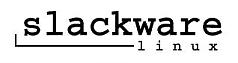
\includegraphics[scale=0.35]{slackware_logo.eps}}

SLS เป็นดิสทริบิวชันค่ายแรกๆแต่ก็ยังเป็นเรื่องยากสำหรับผู้ใช้ทั่วไปที่ติดตั้งและเริ่มต้นใช้ลินุกซ์. นาย Patrick Volkerding\index{general}{patrick volkerding@Patrick Volkerding} เป็นผู้ที่แก้จุดอ่อนเหล่านี้และสร้างดิสทริบิวชันที่มีชื่อว่า {\em Slackware}\index{general}{slackware@Slackware} ขึ้นมาในราวเดือนมิถุนายน ค.ศ.1993. ในเวลาต่อมาดิสทริบิวชันนี้ก็กลายเป็นต้นแบบดิสทริบิวชั่นของค่ายอื่นๆต่อมา. Slackware เน้นความเรียบง่ายของระบบและคำนึงถึงการใช้งาน. โปรแกรมต่างๆที่รวมอยู่ในดิสทริบิวชั่นนี้แพ็กอย่างง่ายๆด้วยโปรแกรม \cmd{tar} และ \cmd{gzip}.


\subsection{{\latintext Red Hat}}\index{general}{redhat@Red Hat}%\marginpar{\includegraphics[scale=0.65]{redhat_logo.eps}}

ในราวปี ค.ศ.1994 \cite{redhathist}, Red Hat เป็นดิสทริบิวชันเชิงพาณิชย์แรกๆที่โปรแกรมติดตั้งใช้ง่ายและเป็น {\em Graphical User Interface (GUI)}. ด้วยเหตุนี้เองที่ทำให้ Red Hat เป็นที่นิยมกันอย่างแพร่หลาย. Red Hat มีจุดเด่นที่{\em การจัดการแพ็กเกจ (Package Management)}, โปรแกรมติดตั้งและ{\em โปรแกรมช่วยควบคุมระบบ (System Management Utilities)}. 

Red Hat ใช้โปรแกรมจัดการแพ็กเกจที่เรียกว่า {\em RPM (Red Hat Package Management)}\index{general}{rpm@RPM|see{Red Hat Package Management}}.\index{general}{redhat package management@Red Hat Package Management} ผู้ใช้สามารถติดตั้งโปรแกรมที่มาในรูปของไฟล์ \cmd{.rpm}. โปรแกรม {\latintext\cmd{rpm}} จะจัดการติดตั้ง{\em ไบนารีไฟล์ (binary file)}, ไฟล์ที่เกี่ยวข้องกับตัวโปรแกรม, คู่มือการใช้งานที่อยู่ในไฟล์ {\latintext\cmd{.rpm}} ไปไว้ในไดเรกทอรี่ที่เหมาะสม. หลักจากที่ติดตั้งไฟล์ต่างๆแล้ว {\latintext\cmd{rpm}} จะ{\em ปรับแต่ง (configure)} ตัวโปรแกรมให้ให้เข้ากับระบบคอมพิวเตอร์และบันทึกข้อมูลที่เกี่ยวกับโปรแกรมนั้นๆใน{\em ฐานข้อมูลการจัดการแพ็กเกจ (Package Management Database)}. ผู้ใช้สามารถ{\em อันอินสตอลล์ (uninstall)} โปรแกรมที่ไม่ต้องการออกจากระบบได้อย่างง่ายดายด้วยโปรแกรม {\latintext\cmd{rpm}} เช่นกัน. ระบบจัดการแพ็กเกจจะลบโปรแกรมและไฟล์ต่างๆที่เกี่ยวข้องให้โดยอัตโนมัติ.
โปรแกรมติดตั้งที่ใช้เป็น GUI ซึ่งสะดวกต่อผู้ที่เริ่มใช้หรือติดตั้งลินุกซ์. หลังจากที่ติดตั้งลินุกซ์แล้ว, ผู้ใช้สามารถปรับแต่งระบบได้ตามที่ต้องการโดยอาศัยยูทิลิตี้โปรแกรมต่างๆ.

Red Hat เป็นดิสทริบิวเชิงพาณิชย์แต่ในขณะเดียวกันอนุญาติให้ผู้ใช้หรือใครก็ได้ดาว์นโหลดทั้งรหัสต้นฉบับ, โปรแกรมติดตั้ง, และแพ็กเกจไบนารีต่างๆ และมีบริการแก้ไขแพ็กเกจที่มีข้อบกพร่องแจกจ่ายด้วย. กล่าวคือผู้ที่ต้องใช้ Red Hat ไม่จำเป็นต้องซื้อแผ่นซีดีจาก Red Hat ก็สามารถใช้ Red Hat ได้, ถ้า Red Hat ที่ใช้อยู่มีช่องโหว่เกี่ยวกับความปลอดภัยก็สามารถอัปเดทแพ็กเกจได้โดยไม่เสียค่าใช้จ่าย. 

เมื่อปลายปี ค.ศ. 2003 ทาง Red Hat \cite{eol} ได้ประกาศการหมดอายุ (end of life) ของ Red Hat Linux 7.1, 7.2, 7.3 และ 8.0. การประกาศมีเนื้อหาเกี่ยวกับการหยุดให้บริการอัปเดท, หยุดการให้บริการ, หยุดการสร้างแพ็กเกจแก้ไขข้อบกพร่องของ Red Hat Linux รุ่นที่ต่ำกว่า 8.0 ภายในสิ้นปี ค.ศ. 2003. และ Red Hat Linux 9 จะหมดอายุขัยภายในเดือนเมษายนปี ค.ศ. 2004. ผู้ใช้ที่ต้องการใช้และบริการอัปเดทต่างๆของ Red Hat ต้องใช้ Red Hat Enterprise Linux ซึ่งจะไม่แจกจ่ายแพ็กเกจไบนารีหรือโปรแกรมติดตั้งต่างๆทางอินเทอร์เน็ต. Red Hat หันมาเน้นธุรกิจทางด้านการให้บริการมากกว่าการขายตัวแพ็กเกจ. ผู้ที่ต้องการใช้ Red Hat Enterprise Linux ต้องเข้าระบบบริการของ Red Hat ซึ่งจะมีหลายระดับตั้งแต่บริการแพ็กเกจแก้ไขโปรแกรมหากมีข้อบกพร่อง, ติดต่อสอบถามทางโทรศัพท์, หรือบริการถึงที่ ฯลฯ \cite{rhel}.

นอกจาก Red Hat Enterprise Linux แล้ว Red Hat ยังเป็นแกนนำสนับสนุนพัฒนาดิสทริบิวชันใหม่ในชื่อ Fedora \cite{fedora} ซึ่งเปิดกว้างให้ผู้สนใจช่วยกันพัฒนาเป็นดิสทริบิวชันเสรีแทน Red Hat Linux ที่หมดอายุไป.


\subsection{{\latintext Debian GNU/Linux}}\index{general}{debian@Debian}%\marginpar{
\includegraphics[scale=0.35]{debian_logo1.eps}
\includegraphics[scale=0.35]{debian_logo2.eps}}

Debian เป็นดิสทริบิวชันที่พัฒนาโดยอาสาสมัครจากทั่วโลกมีชื่อเป็นทางการว่า {\em Debian GNU/Linux}. Debian ถือกำเนิดโดยนาย Ian Murdock เมื่อวันที่ 16 สิงหาคม ค.ศ.1993. นาย Ian ต้องการที่จะทำให้ดิสทริบิวชันที่เขาเริ่มเปิดเผยและมีอุดมการณ์ตามแบบลินุกซ์และ GNU. การสร้างดิสทริบิวชันนี้ได้รับทุนจาก Free Software Foundation เป็นเวลาหนึ่งปีตั้งแต่เดือนพฤศจิกายนปี ค.ศ.1994 ถึงเดือนพฤศจิกายนปีถัดไป \cite{debianhistory}. ชื่อของ Debian (Deb-ian) มาจากชื่อของภรรยาเขาที่มีชื่อว่า Deborah และชื่อของเขาเอง Ian รวมกันเป็นชื่อดิสทริบิวชัน.
 
จุดเด่นของ Debian คือเป็นดิสทริบิวชันที่ไม่หวังผลกำไร, เปิดเผยและให้โอกาสกับนักพัฒนาทุกคนที่สนใจร่วมพัฒนาดิสทริบิวชัน. มีโปรแกรมอำนวยความสะดวกที่เกี่ยวกับการจัดการแพ็กเกจดีเยี่ยมได้แก่ \underline{A}dvanced \underline{P}ackage Managemen\underline{t} หรือเรียกสั้นๆว่า APT.\mymemo{โปรแกรมจัดการแพ็กเกจหลักของระบบจัดการแพ็กเกจ APT ได้แก่ \cmd{apt-get}, \cmd{apt-cache} ฯลฯ.} สิ่งที่เป็นอุปสรรคสำหรับผู้ใช้ใหม่ได้แก่การติดตั้งซึ่งโปรแกรมติดตั้งจะเป็นเมนูแบบเท็กซ์โหมดและในขณะติดตั้งจะมีการถามคำถามเกี่ยวกับการปรับแต่งโปรแกรมต่างๆที่เลือกติดตั้งด้วย. ถ้าผู้ใช้ที่ไม่คุ้นเคยกับลินุกซ์อาจจะไม่เข้าใจทำให้ไม่สามารถตอบคำถามได้เหมาะสม. อย่างไรก็ตามผู้ที่ใช้ Debian มักจะติดตั้งตัวระบบปฏิบัติการเพียงครั้งเดียวและใช้ระบบจัดการแพ็กเกจ APT อัปเกรดระบบปฏิบัติการให้ทันสมัยอยู่เสมอ. ผู้ใช้ไม่จำเป็นต้องติดตั้งระบบทั้งหมดใหม่เมื่อ Debian ประกาศออกตัวรุ่นล่าสุด. 

เมื่อติดตั้ง Debian แล้วผู้ใช้สามารถเลือกประเภทของ Debian ตามการใช้งานได้สามแบบได้แก่
\begin{description}
\item[Stable] \mbox{}\\
เป็นระบบที่รวบรวมแพ็กเกจซอฟต์แวร์ต่างๆที่เสถียรและมีการรับรองเป็นทางการจากทีม Debian หากมีจุดบกพร่องด้านความปลอดภัยหรือข้อผิดพลาดอื่นๆ, จะมีการออกแพ็กเกจอัปเดทแก้ไขให้. คำว่า\emph{เสถียร (stable)} ในที่นี้หมายถึงซอฟต์แวร์แพ็กเกจต่างๆที่อยู่ในระบบได้รับการทดสอบ, ตรวจสอบอย่างถี่ถ้วนก่อนจะรวมแพ็กเกจนั้นๆรวมเป็นระบบ. ทำให้แพ็กเกจที่อยู่ในระบบ stable มีข้อบกพร่องหรือ\emph{บั๊ก (bug)} %
\myvocab{b}{bug}{\emph{บั๊ก}, \emph{ข้อบกพร่อง}. ข้อบกพร่องของซอฟต์แวร์หลังจากที่เจ้าของซอฟต์แวร์นั้นประกาศออกตัวซอฟต์แวร์นั้น}%
น้อยที่สุด. ถ้ามีการพบข้อผิดพลาดอย่างร้ายแรงเช่นข้อผิดพลาดด้านความปลอดภัยของตัวซอฟต์แวร์ก็จะมีการออกแพ็กเกจอัปเกรดที่ได้รับการแก้ไขแล้วโดยที่เลขรุ่นหลักของซอฟต์แวร์ที่ใช้ยังเป็นรุ่นเดิม, ไม่ใช่การเปลี่ยนแพ็กเกจไปใช้รุ่นใหม่. ในกรณีนี้มีข้อดีที่ว่าการใช้งานของซอฟต์แวร์ต่างๆไม่ว่าจะเป็นวิธีการใช้หรือการปรับแต่งยังเหมือนเดิมเพราะเป็นซอฟต์แวร์รุ่นเดิมที่เคยใช้. ดังนั้นระบบแบบ stable จึงเหมาะสำหรับการใช้งานแบบเซิร์ฟเวอร์. 

ในทางกลับกัน, ซอฟต์แวร์ที่เสถียรมีความหมายเป็นนัยว่าซอฟต์แวร์นั้นเป็นรุ่นค่อนข้างเก่า. ซอฟต์แวร์ที่พึ่งออกเผยแพร่ถึงแม้จะมีคุณสมบัติใหม่ๆน่าใช้แต่อาจจะมีข้อบกพร่องซึ่งยังค้นไม่พบอยู่มากจึงถือว่าไม่เสถียร. ด้วยเหตุนี้เองทำให้แพ็กเกจต่างๆที่รวมอยู่ในระบบ stable จึงค่อนข้างเก่าเมื่อเทียบกับระบบแบบอื่น.

\item[Testing] \mbox{}\\
เป็นระบบที่รวมแพ็กเกจที่ผ่านการทดสอบมาระดับหนึ่งจาก unstable และแพ็กเกจต่างๆเหล่านี้มีข้อบกพร่องหรือบั๊กน้อยพอที่จะเป็นตัวแทนแพ็กเกจที่จะเป็นระบบ stable ต่อไป. ระบบนี้เหมาะสำหรับผู้ที่ต้องการใช้ซอฟต์แวร์รุ่นใหม่ๆและเสถียรระดับหนึ่ง. อาจจะใช้เป็นระบบเดกสท็อปก้ำกึ่งกับเซิร์ฟเวอร์ซึ่งมีความจำเป็นต้องการซอฟต์แวร์รุ่นใหม่ๆแต่ไม่ต้องใหม่มากที่สุด.
\item[Unstable] \mbox{}\\
เป็นระบบที่มีแพ็กเกจใหม่ๆรุ่นล่าสุดซึ่งไม่มีการรับประกันว่าจะใช้ได้ดีตามที่คาดหวัง. บางแพ็กเกจอาจจะยังมีข้อบกพร่องที่ต้องแก้ไข. ระบบนี้มีชื่อว่า unstable ซึ่งแปลความหมายว่า ``ไม่เสถียร'' แต่ก็ไม่ได้หมายความไม่เสถียรจริงๆและใช้งานไม่ได้. ระบบนี้เหมาะสำหรับผู้ที่ต้องการใช้ซอฟต์แวร์รุ่นใหม่ล่าสุดและต้องการทดลองความสามารถใหม่ๆของซอฟต์แวร์นั้นๆ.
\end{description}

\subsubsection{ชื่อรหัสการพัฒนา}
ระบบแต่ละแบบจะมี{\emph{ชื่อรหัสการพัฒนา (code name)}\gindex{code name}\gindex{ชื่อรหัสการพัฒนา} ซึ่งนำมาจากชื่อตัวละครในภาพยนตร์การ์ตูนเรื่อง Toy Story. ปัจจุบันระบบ stable มีชื่อรหัสการพัฒนาว่า Sarge, testing มีชื่อว่า ???  และ unstable มีชื่อว่า Sid. ชื่อรหัสการพัฒนาของ unstable จะไม่เปลี่ยนแปลงและเรียกว่า Sid เสมอ. ส่วนชื่อรหัสการพัฒนาของระบบอื่นๆจะเปลี่ยนไปเรื่อยๆเมื่อมีการเลื่อนขั้นเช่น Sarge เป็นชื่อรหัสการพัฒนาของ testing มาก่อน. เมื่อระบบมีความเสถียรเป็นที่ยอมรับจึงเลื่อนขั้นมาเป็น stable แต่ยังมีชื่อรหัสเป็น Sarge เหมือนเดิม. ส่วน testing จะมีการตั้งชื่อใหม่ต่อไป.


\subsection{{\latintext Gentoo}}\index{general}{gentoo@Gentoo}%\marginpar{
\includegraphics{gentoo-tiny.eps}}

Gentoo เป็นดิสทริบิวชันที่ค่อนข้างใหม่ประกาศตัวครั้งแระประมาณเดือนมีนาคมปี ค.ศ.2002. ดิสทริบิวชันนี้มีเอกลักษณ์ที่โดดเด่นแตกต่างจากดิสทริบิวชันอื่นที่ตัวแพ็กเกจเองเป็นรหัสต้นฉบับของซอฟต์แวร์ที่ต้องการติดตั้ง, มีระบบการจัดการแพ็กเกจดีเยี่ยมและมีความยืดหยุ่นสูงในการปรับแต่งระบบ. 

Gentoo มีระบบการควบคุมแพ็กเกจที่เรียกว่า \emph{portage}\mymemo{โปรแกรมจัดการแพ็กเกจหลักของระบบควบคุมแพ็กเกจ Portage ได้แก่ \cmd{emerge} และ \cmd{ebuild}.} \index{general}{portage}ซึ่งได้รับแนวคิดมาจากระบบ port ของยูนิกซ์ BSD. ระบบควบคุมแพ็กเกจนี้สามารถค้นหา, ดาว์นโหลด, แก้ไขความขึ้นกับแพ็กเกจอื่นๆ (package dependency) และติดตั้งแพ็กเกจที่ต้องการได้โดยอัตโนมัติเช่นเดียวกับระบบ APT ของ Debian. แพ็กเกจของ Gentoo ไม่ใช่ตัวโปรแกรม, ไม่ใช่รหัสต้นฉบับแต่เป็นไฟล์สคริปต์บอกว่ารหัสต้นฉบับอยู่ที่ไหน, มีข้อมูลของวิธีคอมไพล์และติดตั้ง. การติดตั้งแพ็กเกจมีขั้นตอนต่างๆได้แก่การดาว์นโหลดรหัสต้นฉบับ, การตรวจสอบความสัมพันธ์กับแพ็กเกจอื่นๆ, คอมไพล์และติดตั้ง. ในช่วงของการคอมไพล์, ผู้ใช้สามารเลือกปรับแต่งค่าต่างๆที่อาจจะมีผลต่อประสิทธิภาพการทำงานเช่นตัวเลือกคอมไพล์ให้เหมาะกับหน่วยประมวลผลข้อมูลที่ใช้, หรือปรับตัวเลือกตอนสร้างของแพ็กเกจนั้นๆให้เหมาะสมตามที่ต้องการได้. 

การจัดการแพ็กเกจแบบนี้อาจจะเสียเวลากับการคอมไพล์ถ้าเป็นแพ็กเกจที่ใหญ่แต่มีข้อดีที่สามารถปรับแต่งแพ็กเกจหรือระบบได้จากรหัสต้นฉบับ. การปรับแต่งได้จากรหัสต้นฉบับต้นฉบับนี่เองที่ต่างจากดิสทริบิวชันอื่นที่แพ็กเกจเป็นไพล์ไบนารีที่คอมไพล์ไว้เรียบร้อยแล้วซึ่งแพ็กเกจไบนารีเหล่านี้สร้างมาสำหรับคอมพิวเตอร์ทั่วไปไม่ได้เฉพาะเจาะจง. 

หลังจากที่ติดตั้ง Gentoo แล้ว, ผู้ใช้สามารถเลือกระบบได้สองประเภทได้แก่
\begin{description}
\item[Stable] \mbox{}\\
เป็นระบบที่รวมแพ็กเกจต่างๆที่เสถียรเหมาะสำหรับการใช้ตั้งแต่เดกสท็อปส่วนบุคคลถึงเซิฟร์เวอร์.
\item[Unstable] \mbox{}\\
เป็นระบบที่รวแพ็กเกจที่ใหม่ล่าสุดซึ่งอาจจะมีบั๊กแต่ไม่ได้หมายความใช้งานไม่ได้. ระบบนี้เหมาะสำหรับผู้ที่ต้องใช้ซอฟต์แวร์รุ่นใหม่ล่าสุด, ทดลองความสามารถใหม่ๆของซอฟต์แวร์เป็นต้น.
\end{description}




\subsection{{\latintext Fedora}}\index{general}{fedora@Fedora}%\marginpar{
\includegraphics[scale=0.9]{fedora_logo.eps}}

Fedora เดิมเป็นโครงการสร้างแพ็กเกจสำหรับใช้ร่วมกับ Red Hat โดยกลุ่มอาสมัครในอินเทอร์เน็ต \cite{fedora_original}. โครงการนี้เปิดกว้างให้ใครก็ได้ที่สนใจเข้าร่วมโครงการก็ได้โดยไม่หวังผลกำไรคล้ายกับชุมชนของนักพัฒนา Debian แต่ Fedora เป็นดิสทริบิวชันที่มาฐานมาจาก Red Hat.

ในปีค.ศ.2003, Red Hat ประกาศเลิกสนับสนุน Red Hat ที่แจกจ่ายฟรีโดยเปลี่ยนแนวทางมาสนับสนุน Red Hat ที่เป็นสินค้าจำหน่ายเช่น Red Hat Enterprise โดยที่ผู้ต้องการสนับสนุนจาก Red Hat ต้องเสียค่าใช้จ่าย. เพื่อเป็นการสนับสนุนชุมชนโอเพนซอร์สต่อไป, Red Hat จึงตัดสินใจเลือกโครงการ Fedora ทำเป็นดิสทริบิวชันต่อจาก Red Hat โดยที่ทาง Red Hat เป็นผู้สนับสนุนอย่างเป็นทางการ. 

จุดเด่นของ Fedora ได้แก่การเป็นดิสทริบิวชันสร้างจาก Red Hat แต่เปิดกว้างในการพัฒนานาแก่สาธารณะและนำระบบการจัดการแพ็กเกจชั้นสูงของดิสทริบิวชันอื่นมาใช้ด้วยได้แก่ APT และ \cmd{yum}. โดยสภาพรวมทั่วไปแล้วยังคงเหมือนกับ Red Hat.


\subsection{{\latintext Knoppix}}\index{general}{knoppix@Knoppix}%\marginpar{\includegraphics[scale=0.8]{knoppix.eps}}
สำหรับผู้ต้องการลองใช้ลินุกซ์แต่ยังไม่พร้อมที่จะอินสตอลล์ลงในฮาร์ดดิกส์, Knoppix เป็นทางเลือกสำหรับกรณีนี้. Knoppix เป็นแผ่น CD ที่บูตได้, รวบรวมลินุกซ์เคอร์เนลและโปรแกรมเดกสท็อปที่จำเป็นไว้ในแผ่นซีดีแผ่นเดียวโดยมีฐานจาก Debian. แผ่นซีดีนี้สามารถค้นหาฮาร์ดแวร์และอินสตอลล์ไดร์เวอร์ให้โดยอัตโนมัติ. ผู้ใช้เพียงแค่บูตเครื่องคอมพิวเตอร์ด้วยแผ่นซีดี Knoppix ก็จะสามารถใช้โปรแกรมต่างๆบนลินุกซ์เช่น KDE, Mozilla, Gimp ฯลฯ. แผ่นซีดีนี้สามารถใช้เป็นแผ่นทดลองหรือจะใช้เป็นแผ่นซีดีกู้ภัยเครื่องคอมพิวเตอร์ก็ได้ในกรณีที่คอมพิวเตอร์ไม่สามารถบูตจากฮาร์ดดิกส์. บางคนใช้ Knoppix เป็นตัวทดสอบก่อนที่จะซื้อเครื่องคอมพิวเตอร์ว่าใช้ลินุกซ์ได้หรือไม่โดยถือแผ่นซีดีไปลองที่ร้าน.

ถ้าลองใช้ Knoppix ไปสักระยะหนึ่งแล้วต้องการติดตั้งลงในฮาร์ดิกส์ก็สามารถทำได้โดยสั่งคำสั่ง \cmd{knx-hdinstall} ซึ่งจะแสดงหน้าจอเมนูช่วยแนะนำขั้นตอนต่างๆในการติดตั้ง. เนื่องจาก Knoppix พัฒนาจาก Debian, หลังจากติดตั้งเรียบร้อยแล้วก็สามารถใช้คำสั่ง \cmd{apt-get} และจัดการระบบได้ทุกอย่างเหมือน Debian.

ช่วงต้นเดือนมีนาคม ค.ศ.2004 คุณ ภัทระ เกียรติเสรี, สมาชิก TLWG ได้ปรับแต่ง Knoppix ให้มีสภาพแวดล้อมเป็นภาษาไทยและใช้ภาษาไทยได้โดยปริยาย \cite{knoppix-th}. นอกจากนี้ยังมีเพิ่มซอฟต์แวร์ภาษาไทยที่น่าใช้ต่างๆด้วยเช่น NECTEC LEXiTEON Dictionary \cite{lexitron}, NECTEC Arnthai OCR software \cite{arnthai}, Thai \LaTeX{} เป็นต้น.


\bigskip
นอกจากดิสทริบิวชั่นที่กล่าวแล้ว ยังมีดิสทริบิวชั่นอีกหลายค่ายเช่น  Suse, Mandriva\mymemo{ชื่อเดิมของ Mandriva คือ Mandrake}, Turbolinux ฯลฯ. ผู้อ่านสามารถหาข้อมูลเกี่ยวกับดิสทริบิวชันต่างๆได้จากโฮมเพจของ DistroWatch.com \cite{distrowatch} ซึ่งเป็นแหล่งรวมข้อมูลของดิสทริบิวชันต่างๆที่มีอยู่ทั่วโลกตั้งแต่ดิสทริบิวชันค่ายใหญ่จนถึงค่ายเล็ก.
%\begin{figure}
%\plfigure{.5}{distribution.eps}{เปรียบเทียบช่วงเวลารีลีสของเคอร์เนลและดิสทริบิวชั่นค่ายต่างๆ}%{linuxtimeline}
%\end{figure}


%\marginpar{\scalebox{.9}{
\includegraphics{images/suse_logo.eps}}}
%\marginpar{\scalebox{.45}{\includegraphics{images/turbolinux_logo.eps}}}
%\marginpar{\scalebox{.35}{
\includegraphics{images/mandrake_logo.eps}}}
%\marginpar{\scalebox{.35}{
\includegraphics{images/tle_logo.eps}}}

\section{ลินุกซ์ดิสทริบิวชันในประเทศไทย}
\begin{description}
\item[Linux TLE (ทะเล)]\mbox{}\\
Linux TLE ย่อมาจากคำว่า Linux Thai Language Extension \cite{opentle} เป็นดิสทริบิวชันที่พัฒนาโดยศูนย์เทคโนโลยีอิเล็กทรอนิกส์และคอมพิวเตอร์แห่งชาติ (NECTEC). มุ่งเน้นการใช้งานภาษาไทยกับลินุกซ์ด้านเดกสท็อป. ประกอบด้วยโปรแกรมใช้งานทั่วไปที่สนับสนุนภาษาไทย ได้แก่ออฟฟิสทะเล, โปรแกรมอ่านอีเมลล์, บราวเซอร์ ฯลฯ. 

ลินุกซ์ทะเลเดิมพัฒนามาจาก Mandrake และเปลี่ยนมาพัฒนาจาก Red Hat ในเวลาต่อมา. Linux TLE รุ่นล่าสุด\mymemo{Linux TLE รุ่นล่าสุดขณะที่เขียนหนังสือเล่มนี้ได้แก่รุ่น 5.5.}พัฒนามาจาก Fedora.
\item[Burapha Linux (บูรพาลินุกซ์)]\mbox{}\\
เป็นดิสทริบิวชันไทยที่สร้างโดยคณะวิทยศาตร์ภาคคอมพิวเตอร์ของมหาวิทยาลัยบูรพา. เป็นดิสทริบิวชันที่พัฒนามาจาก Slackware เพื่อให้นักศึกษาเรียนรู้และทำความเข้าใจเกี่ยวกับระบบปฏิบัติการยูนิกซ์ \cite{burapha}. 
\end{description}

นอกจากดิสทริบิวชันที่แนะนำไปแล้วยังมีดิสทริบิวชันไทยอื่นๆด้วยเช่น Grand Linux เป็นดิสทริบิวชันเชิงพาณิชย์และให้บริการกับดิสทริบิวชันในรูปแบบต่างๆ.

%จากการสังเกตุของผู้เขียนเองการพัฒนาของดิสทริบิวชันในเมืองไทยที่เรียกได้ว่าเปิดกว้างมากที่สุดได้แก่ Linux TLE สามารถดาว์นโหลดได้แรกเปลี่ยนความรู้กันได้ระดับหนึ่ง. 

\section{Thai Linux Working Group}
นอกจากลินุกซ์ดิสทริบิวชันไทยแล้ว, ในประเทศไทยมีกลุ่มชุมชนบนอินเทอร์เน็ตที่ชื่อ \emph{Thai Linux Working Group (TLWG)}\index{general}{thai linux working group@Thai Linux Working Group}\index{general}{tlwg@TLWG|see{Thai Linux Working Group}} \cite{tlwg}. TLWG เป็นกลุ่มของผู้ใช้และพัฒนาซอฟต์แวร์บนลินุกซ์ไม่จำกัดว่าต้องเป็นดิสทริบิวชันใด. TLWG ก่อตั้งขึ้นมาโดยมีจุดประสงค์เพื่อ
\begin{itemize}
\item \mymemo{คัดลอกมาจากเว็บไซด์ \cite{tlwg} โดยตรง}แลกเปลี่ยนความคิดเห็น และสร้างสรรค์ผลงานที่จะผลักดันให้การใช้งานลินุกซ์ของคนไทยเป็นไปได้อย่างมีประสิทธิภาพ, และถูกต้องตามมาตรฐาน.
\item สนับสนุนให้การพัฒนาต่างๆในแง่ที่มีผลกับคนไทยโดยรวม, เป็นไปอย่างเปิดเผย.
\end{itemize}

สมาชิกสามารถสนทนาแสดงความคิดเห็น, ถามตอบ ในเรื่องเกี่ยวกับการใช้งานทั่วไป, การพัฒนาซอฟต์แวร์บนลินุกซ์ ตลอดจนสัพเพเหระได้ผ่านเว็บบอร์ด, mailing list หรือนิวส์กรุป. เว็บไซด์ของ TLWG ที่เรียกย่อๆว่า LTN (\underline{l}inux.\underline{t}hai.\underline{n}et)ได้รับการสนับสนุนจากศูนย์เทคโนโลยีอิเล็กทรอนิกส์แห่งชาติ และ Internet Thailand. กิจกรรมและบริการของ TLWG ได้แก่
\begin{description}
\item[เว็บบอร์ด] \mbox{}\\
เว็บบอร์ดเป็นที่ถามตอบให้แก่ผู้สนใจได้แก่ เว็บบอร์ดเกี่ยวกับลินุกซ์ทั่วไป, เว็บบอร์ดเกี่ยวกับการพัฒนาซอฟต์แวร์บนลินุกซ์ และเว็บบอร์ดอื่นๆที่ไม่เข้าข่ายเว็บบอร์ดทั้งสองชนิดข้างต้น.
\item[Mailing list] \mbox{}\\
Mailing list มีเนื้อหาเหมือนกับเว็บบอร์ด, เสนอเนื้อหาในรูปของอีเมลล์เท่านั้น. Mailing list ของ Tlwg เป็นบริการของ yahoogroup.com.
\item[Newsgroup] \mbox{}\\
นิวส์กรุปมีเนื้อหาเหมือนกับเว็บบอร์ด, เสนอเนื้อหาในรูปของนิวส์กรุปโดยมีเซิฟร์เวอร์อยู่ที่ thaigate.nii.ac.jp.
\item[ข่าว] \mbox{}\\
ผู้สนใจสามารถโพสข่าวที่เกี่ยวกับลินุกซ์ขึ้นโฮมเพจหน้าแรกได้. ผู้ดูแลโฮมเพจจะอนุมัติให้ข่าวที่โพสลงในโฮมเพจได้ถ้าเห็นว่าเนื้อหาเหมาะสม.
\item[บทความโดย TLWG หรือสมาชิก] \mbox{}\\
TLWG บริการเนื้อที่สร้างโฮมเพจสำหรับผู้ลงทะเบียนไว้. ผู้ที่สนใจสามารถเขียนบทความที่เกี่ยวกับลินุกซ์เพื่อเป็นประโยชน์สำหรับคนอื่นๆได้.
\item[CVS] \mbox{}\\
\myvocab{c}{CVS}{\emph{Concurrent Versions Systems}. เป็นระบบที่ช่วยเก็บและควบคุมเวอร์ชันของรหัสต้นฉบับ. มีประโยชน์อย่างยิ่งโดยเฉพาะการพัฒนาซอฟต์แวร์ร่วมกันหลายคนโดยผ่านทางเน็ตเวิร์ก, ไม่มีข้อจำกัดเรื่องที่อยู่ของนักพัฒนาซอฟต์แวร์.}ซอฟต์แวร์ที่ดูแลและพัฒนาโดย TLWG เช่น thailatex, thaifonts-scalable จะเก็บไว้ในเซิฟร์เวอร์โดยใช้ระบบ CVS. ผู้สนใจสามารถใช้คำสั่ง \cmd{cvs} เพื่อนำซอฟต์แวร์รุ่นที่ต้องการมาใช้ได้.
\item[Ftp] \mbox{}\\
บริการ ftp ให้บริการดาว์นโหลดซอฟต์แวร์หรือเอกสารต่างๆที่เกี่ยวกับลินุกซ์.
\end{description}






\section{ลินุกซ์และยูนิกซ์}

\begin{figure}[!b]
\plfigure{0.8}{unix_time.eps}{ระบบปฏิบัติการตระกูลยูนิกซ์}{unixhis}
\end{figure}
ถ้าพูดถึงระบบปฏิบัติการลินุกซ์แล้วคงหลีกเลี่ยงที่จะพูดถึงระบบปฏิบัติการยูนิกซ์ด้วยไม่ได้เพราะลินุกซ์เป็นระบบปฏิบัติการตระกูลยูนิกซ์ประเภทหนึ่ง. เพื่อให้ผู้อ่านเข้าใจลินุกซ์มากยิ่งขึ้นจึงแนะนำเรื่องราวเกี่ยวกับระบบปฏิบัติการยูนิกซ์ในช่วงนี้ด้วย.

ลินุกซ์สามารถทำทุกอย่างที่ยูนิกซ์ทำได้, มี{\em คำสั่ง (command)} และ{\em ซิสเต็มคอลล์ (system call)}\myvocab{s}{system call}{\emph{ซิสเต็มคอลล์}. ฟังค์ชันภาษาซีสำหรับติดต่อใช้งานเคอร์เนล.} เหมือนๆกัน.
% ลินุกซ์ มีหลักการเหมือนยูนิกซ์ที่ว่าผู้ใช้ไม่สามารถใช้เคอร์เนลได้โดยตรง ต้องส่งผ่านคำสั่งให้ kernel
%ผ่านทาง shell, มี system calll เหมือนกันเป็นต้น. 
สิ่งที่ลินุกซ์แตกต่างจากยูนิกซ์คือ, ลินุกซ์เป็นซอฟต์แวร์เสรีและรหัสต้นฉบับที่เขียนด้วยภาษา C ไม่ได้ลอกเลียนรหัสต้นฉบับของยูนิกซ์ที่มีอยู่แต่เดิม. 

ผู้อ่านอาจจะตั้งคำถามว่าทำไมลินุกซ์จึงสร้างเลียนแบบระบบปฏิบัติการยูนิกซ์ทั้งๆที่มีระบบปฏิบัติอื่นๆอีกมากมาย. คำตอบคือเพราะยูนิกซ์เป็นระบบปฏิบัติการที่ออกแบบอย่างดี, มีปรัชญา (UNIX Philosophy) ที่ว่าสร้างระบบปฏิบัติการที่ไม่ใหญ่เกินไป, ทำงานเท่าที่จำเป็น, โปรแกรมต่างๆสามารถส่งผลลัพธ์ให้โปรแกรมอื่นต่อได้. ในช่วงต่อไปนี้จะกล่าวถึงประวัติความเป็นมาของระบบปฏิบัติการยูนิกซ์ \cite{magicgarden,newfrontier,osbook1} เพื่อให้ผู้อ่านได้รู้จักยูนิกซ์และเข้าใจพื้นฐานของลินุกซ์ได้ดียิ่งขึ้น.

\subsection{กำเนิด  UNIX}
คอมพิวเตอร์ในยุคแรกแตกต่างจากคอมพิวเตอร์ในปัจจุบัน. คอมพิวเตอร์ในยุคแรกเหมือนกับเครื่องคิดเลขขนาดใหญ่ ทำงานได้อย่างเดียวและใช้ได้คนเดียว. ผู้ใช้ซึ่งส่วนใหญ่เป็นนักวิจัยสั่งงานโดยป้อนชุดคำสั่งที่เรียกว่าโปรแกรมผ่านทางเทปหรือ{\em พันช์การ์ด (pucnh card)}. เมื่อใช้งานเสร็จแล้วผู้ใช้คนต่อไปทำสิ่งเดียวกันคือป้อนข้อมูล, รอคอมพิวเตอร์ทำงาน, รอรับผลที่จะบันทึกกลับลงในเทป. การใช้งานคอมพิวเตอร์ในลักษณะนี้ทำให้เกิดปัญหาหลายอย่างเช่น ในกรณีที่มีผู้ใช้หลายคน คอมพิวเตอร์ไม่สามารถให้บริการได้, การใช้งานแต่ละครั้งมีเสียค่าใช้จ่ายสูงเป็นต้น. จากสาเหตุดังกล่าวจึงเกิดความคิดเกี่ยวกับการสร้างระบบปฏิบัติการขึ้น. ผู้ใช้งานจะสั่งให้คอมพิวเตอร์ทำงานโดยผ่านตัวระบบปฏิบัติการ.

ในปีค.ศ. 1965, Massachusetts Institute of Technology (MIT), Bell Telephone Laboratories (BTL)
%\mymarginpar{ Bell Laboratory: ศูนย์วิจัยของบริษัท  AT\&T,
%ผลงานวิจัยและสิ่งประดิษฐ์ที่มีคุณค่าแก่โลกหลายชิ้นกำเนิดมาจากศูนย์วิจัยแห่งนี้เช่น  transistor เป็นต้น} 
และ General Electrics Company (GE) ร่วมกันพัฒนาระบบปฏิบัติการแบบ time-sharing ที่เรียกว่า MULTICS (MULtiplexed Information and Computing Service)\index{general}{multics@MULTICS}. ในปีค.ศ. 1969 BTL ตัดสินใจถอนตัวจากโครงการดังกล่าว แต่ผู้ร่วมโครงการดังกล่าวจาก BTL ได้แก่ Ken Thompson, Dennis Ritchie, Doug McIlroy, และ J. F. Ossanna\index{general}{ken thopmson@Ken Thompson}\index{general}{dennis ritchie@Dennis Ritchie} ยังรอคอยโอกาสที่จะได้พัฒนาระบบปฏิบัติการในโอกาสหน้า. พวกเขาตั้งใจที่จะพัฒนาระบบปฏิบัติด้วยตัวเอง แต่เนื่องจากคอมพิวเตอร์มีราคาแพงในสมัยนั้น ทำให้ไม่สามารถหาคอมพิวเตอร์ที่จะเอามาทดลองพัฒนาได้. มีความพยายามที่ของบประมาณซื้อคอมพิวเตอร์เพื่อการทดลองแต่ก็ถูกปฏิเสธไป. ถึงแม้ว่าจะไม่สามารถทำการทดลองได้ Thompson, R. H. Canaday, และ Ritchie ได้พัฒนาช่วยกันออกแบบ file system ในทางทฤษฎี. 

ในปีค.ศ. 1969, Thompson สร้างเกมส์ ``Space Travel''. เกมส์นี้สร้างบนระบบปฏิบัติการ Multics แล้วเขียนใหม่ด้วยภาษา Fortran บนระบบปฏิบัติการ  GECOS (ระบบปฏิบัติของ GE ในตอนนั้น)\mymemo{GECOS เป็นระบบปฏิบัติการของเครื่องคอมพิวเตอร์ที่ GE ผลิต. หลังจากนั้น HoneyWell เป็นผู้ขายคอมพิวเตอร์นี้ในช่วงเวลาถัดมา}. ช่วงนี้เองที่ Thompson หาเครื่องคอมพิวเตอร์ PDP-7 ที่ไม่ค่อยมีใครใช้ได้, จึงเป็นโอกาสให้เขาและ Ritchie เขียนโปรแกรม Space Travel ให้ใช้กับเครื่อง PDP-7 ที่เขาหาได้. สิ่งที่เขาทำก้าวหน้าขึ้นเรื่อยๆ, เขาเริ่มสร้าง file system ที่เคยคิดไว้. สร้างยูทิลิตี้ระบบดับยูสเซอร์เช่น copy, print, delete, editor, และ shell. โปรแกรมต่างๆพัฒนาด้วย cross-assembler บน GECOS แล้วย้ายตัวโปรแกรมไปสู่ PDP-7 ด้วยเทปกระดาษ. เมื่อสร้าง assembler สำหรับเครื่อง PDP-7 สำเร็จ, การพัฒนาโปรแกรมต่างๆก็ไม่ต้องอาศัย GECOS อีกต่อไป. มีแค่ shell, editor, และ assembler ก็สามารถสร้างระบบขึ้นมาใหม่ได้ด้วยตัวเอง(ไม่ต้องพึ่งคอมพิวเตอร์เครื่องอื่น).
ต่อมาในปีค.ศ. 1970 Brian Kernighan เรียกระบบปฏิบัติการที่ Thompson และ Ritchie สร้างเลียนแบบ MULTICS ว่า {\bf UNICS} (UNiplexed Information and Computing Service) ซึ่งต่อมากลายเป็นคำว่า {\bf UNIX} นั่นเอง.\index{general}{unix@UNIX}\index{general}{unics@UNICS|see{UNIX}} 

เริ่มแรกยูนิกซ์ใช้ใน{\em งานประมวลข้อความ (text processing)} ในแผนกสิทธิบัตรของ BTL. โปรแกรมที่ใช้ในตอนนั้นได้แก่ \cmd{roff} และ \cmd{ed} เป็นต้น. เนื่องจากยูสเซอร์เพิ่มมากขึ้นและ BTL เริ่มเห็นประโยชน์ของระบบปฏิบัติการนี้จึงอนุมัติการซื้อคอมพิวเตอร์รุ่นใหม่คือ PDP-11 ในเวลาต่อมา. เมื่อยูนิกซ์พอร์ตไปใช้กับเครื่อง PDP-11 ได้สำเร็จ ถือว่าเป็นจุดเริ่มของระบบปฏิบัติการยูนิกซ์อย่างเป็นทางการเรียกว่า UNIX First Edition. ต่อมามีการเพิ่มความสามารถการทำงานต่างๆเรื่อยๆจนออกเป็น Second Edition, Third Edition.

\subsection{จากภาษาแอสเซมบลีสู่ภาษา C}
ยูนิกซ์พอร์ตไปใช้กับเครื่อง PDP-11 ได้ด้วยภาษาแอสเซมบลี. เดิมที Thompson ตั้งใจที่เขียนระบบปฏิบัติการยูนิกซ์ใหม่ด้วย{\em ภาษาชั้นสูง (high-level language)}\index{general}{ภาษาชั้นสูง}\index{general}{high-level language|see{ภาษาชั้นสูง}}\myvocab{h}{high-level language}{\emph{ภาษาชั้นสูง}. หมายถึงภาษาคอมพิวเตอร์ที่มนุษย์อ่านแล้วทำความเข้าใจได้, ไวยกรณ์ไม่ขึ้นกับเครื่องคอมพิวเตอร์ที่ใช้งาน. ตัวอย่างของภาษาชั้นสูงได้แก่ C, C++, Java เป็นต้น.} แทนภาษาแอสเซมบลี. เขาพยายามเขียนระบบปฏิบัติการยูนิกซ์ด้วยภาษา Fortran แต่ก็ล้มเลิกไปในวันแรกที่ลอง. นอกจากนั้น Thompson ยังสร้างภาษาใหม่ที่เรียกว่าภาษา  B (B langauage) เพื่อใช้เขียนระบบปฏิบัติการ แต่มีปัญหาตามมาหลายอย่างเช่น ภาษา B เป็น interpreter ทำให้ทำงานช้าไม่เหมาะกับการเขียนระบบปฏิบัติการเป็นต้น. ต่อมา Ritchie จึงพัฒนาภาษา B ต่อให้เป็นภาษาใหม่ที่เรียกว่าภาษา C. 

ในราวปีค.ศ. 1973 เขาทั้งสองเขียนระบบปฏิบัติยูนิกซ์ใหม่หมดด้วยภาษา C แทนภาษาแอสเซมบลี, ทำให้สามารถพอร์ตตัวระบบปฏิบัติการไปใช้กับคอมพิวเตอร์รุ่นใหม่หรือรุ่นอื่นได้ง่ายขึ้น. ปรากฏการนี้ถือว่าเป็นเรื่องใหม่สำหรับวงการคอมพิวเตอร์เพราะระบบปฏิบัติการสมัยนั้นเขียนด้วย{\em ภาษาชั้นต่ำ (low-level language)}\index{general}{low-level language|see{ภาษาชั้นต่ำ}}\index{general}{ภาษาชั้นต่ำ} เช่นภาษาแอสเซมบลีเป็นต้น. ในตอนนี้ยูนิกซ์ได้ก้าวเข้าสู่ช่วง Fourth Edition แล้ว. ต่อมายูนิกซ์พอร์ตไปใช้กับคอมพิวเตอร์อื่นๆนอกจาก PDP-11 เช่น Interdata 7/32, VAX เป็นต้น

\subsection{Berkeley Software Distribution (BSD)}\index{general}{berkley software distribution@Berkley Software Distribution}\index{general}{bsd@BSD|see{Berkley Software Distribution}}
ในช่วงปีค.ศ. 1976-1977, Thompson ได้รับเชิญจากมหาวิทยาลัย The University of California-Berkeley ให้เป็นศาสตรจารย์พิเศษสอนเกี่ยวกับระบบปฏิบัติการที่เขาสร้าง. และยูนิกซ์ก็เริ่มเป็นที่รู้จักแพร่หลายในวงการศึกษา. ในเวลานั้นนักศึกษามหาวิทยาลัยที่ Berkeley โดยมี Bill Joy\index{general}{bill joy@Bill Joy}\mymemo{ในปีค.ศ. 1982, Bill Joy, และเพื่อนๆอีก 3 คนรวมตัวกันสร้างบริษัท Sun Microsystems ซึ่งเป็นบริษัทชั้นนำในวงการยูนิกซ์ปัจจุบัน} เป็นแกนนำ, สร้างยูทิลิตี้โปรแกรม, แก้ไขเคอร์เนล, และรวบรวมแจกจ่ายในชื่อของ Berkeley Software Distribution (BSD) เมื่อปีค.ศ. 1978. 

ในช่วงนี้ยูนิกซ์พัฒนาไปมาก. Bill Joy สร้างเชลล์ตัวใหม่ที่ชื่อ \cmd{csh} มีความสามารถควบคุม{\em จ็อบ (job)}, มี{\em ฮิสตอรี่ฟังชั่น (history function)} ซึ่งเชลล์ก่อนหน้านี้ไม่มี. นอกจากนั้นเขายังสร้างบรรณาธิกรณ์ \cmd{ex} ซึ่งเปลี่ยนชื่อมาเป็น \cmd{vi}\index{general}{vi@\cmd{vi}}\mymemo{\cmd{vi} อ่านออกเสียงว่า vee-eye (วีอาย)} ภายหลัง. สิ่งที่สำคัญอีกประการหนึ่งคือในช่วงนั้นกระทรวงกลาโหมของอเมริกาสร้างโปรเจค DARPA (Defense Advanced Research Projects Agency)\index{general}{darpa@DARPA} ซึ่งเป็นแกนนำในการสร้างอินเทอร์เน็ต, ให้เงินทุนสนับสนุนการวิจัยที่ Berkeley อย่างมาก มีผลให้ BSD และยูนิกซ์ในรุ่นต่อมาสนับสนุนการใช้โปรโตคอล {\em TCP/IP (Transmission Control Protocol / Internet Protocol)} อย่างกว้างขวาง.

\subsection{UNIX System V}\index{general}{system v@System V}
ในขณะที่ Berkeley พัฒนายูนิกซ์เวอร์ชั่นของตัวเอง, ทางด้าน AT\&T ก่อตั้ง UNIX Support Group (USG) และสนับสนุนยูนิกซ์ในการค้า. AT\&T ออกขายยูนิกซ์ในชื่อ UNIX System III แต่ได้รับการต้อนรับไม่สู้ดีนักเนื่องจากคุณภาพ. ในปีค.ศ. 1983 จึงออกตัวยูนิกซ์ที่ปรับปรุงตัวเคอร์เนลให้มีคุณสมบัติดีขึ้น และเป็นที่รู้จักกันในชื่อของ UNIX System V. หลังจากนั้นมีการปรับปรุงระบบปฏิบัติการให้ดีขึ้นเป็นระยะๆ ในชื่อของ UNIX system V Release 2, 3, และ 4.


\subsection{มาตรฐานยูนิกซ์}
ยูนิกซ์แบ่งออกเป็น 2 ค่ายใหญ่ๆชัดเจนระหว่าง UNIX System V และ BSD. ถึงแม้ว่าจุดเริ่มต้นมาจากที่เดียวกันแต่มีการแก้ไขปรับปรุงรหัสต้นฉบับของเคอร์เนลโดยแต่ละฝ่ายทำให้ยูนิกซ์ทั้งสองไม่มีความเข้ากันได้ (compatibility) ทั้งทางด้านไบนารีและซิสเต็มคอลล์. ซอฟแวร์และฮาร์ดแวร์เวนเดอร์ต่างๆเริ่มขายยูนิกซ์ที่ตนเองสร้างแบ่งตามสาย System V และ BSD. ตัวอย่างเช่น SunOS มีพื้นฐานมาจาก BSD\mymemo{SunOS เป็นระบบปฏิบัติการเก่าของ Sun Microsystem. ปัจจุบันยูนิกซ์ที่ Sun Mucrosystem ใช้คือ Solaris ซึ่งมีรากฐานจาก System V} เป็นต้น. เดเวล็อปเปอร์ที่พัฒนาโปรแกรมบนยูนิกซ์เกิดความลำบากในการเลือกระบบปฏิบัติที่จะใช้. โปรแกรมที่เขียนบน System V อาจจะต้องนำมาแก้ไขเพื่อให้ใช้ได้บน BSD ทั้งๆที่เป็นยูนิกซ์เหมือนกัน. 

ความพยายามที่จะทำให้ยูนิกซ์เป็นมาตรฐานเดียวกันที่เป็นกลางที่สุดได้แก่มาตรฐานของ POSIX (Portable Operating System based on UNIX)\index{general}{posix@POSIX} ที่กำหนดโดยสถาบัน IEEE (The Institute of Electrical and Electronic Engineers). ตัวอย่างเช่นมาตรฐานนี้กำหนดว่ายูนิกซ์ทุกประเภทต้องประกอบด้วยไลบรารี่มาตรฐานที่กำหนดไว้, ซอฟต์แวร์เวนเดอร์แต่ละรายสามารถเพิ่มไลบรารี่ที่เป็นประโยชน์นอกเหนือจากที่กำหนดได้. นอกจากการกำหนดไลบรารี่แล้ว POSIX ยังกำหนดเชลล์, ยูทิลิตี้, ซิสเต็มคอลล์ที่ต้องมีอยู่ในระบบปฏิบัติการยูนิกซ์อีกด้วย.




\section{สรุปท้ายบท}
\begin{itemize}
\item ลินุกซ์ คือระบบปฏิบัติการที่มีคุณสมบัติคล้ายเหมือนกับระบบปฏิบัติการยูนิกซ์ แต่พัฒนาขึ้นมาโดยไม่ได้ลอกเลียนหรือสืบทอดรหัสต้นฉบับของยูนิกซ์. โปรแกรมที่ใช้บน ลินุกซ์ มีความเข้ากันได้กับระบบปฏิบัติการยูนิกซ์อื่นในระดับรหัสต้นฉบับ.
\item ลินุกซ์ สามารถแบ่งเป็นสองส่วนใหญ่ๆคือ {\em เคอร์เนล}และ{\em โปรแกรมใช้งาน}. โปรแกรมใช้งานต่างๆทำงานได้โดยมีเคอร์เนลเป็นพื้นฐานทำหน้าที่ควบคุมการใช้งานของโปรเซสเซอร์, หน่วยความจำ, ดิกส์ ฯลฯ. เคอร์เนลโดยลำพังทำงานเองไม่ได้.
\item แก่นของระบบปฏิบัติการที่เรียกว่าเคอร์เนลเขียนด้วยภาษา C เป็นหลัก. รหัสต้นฉบับของระบบปฏิบัติการเปิดเผยแก่สาธารณะ. ลินุกซ์ ให้อิสระแก่ผู้ใช้ที่จะศึกษา, ดัดแปลง, ก๊อบปี้ ฯลฯ ตราบเท่ารหัสต้นแบบที่เปลี่ยนแปลงเปิดเผยต่อสาธารณะต่อไป.
\item เคอร์เนลและโปรแกรมใช้งานต่างๆพัฒนาหรือพอร์ตโดยเดเวลลอปเปอร์ทั่วโลกโดยอาศัยอินเทอร์เน็ตเป็นสื่อ. ตัวเคอร์เนลและโปรแกรมต่างๆฟรี. ฟรีในที่นี้ไม่ได้ถึงราคาเป็น ``0'' แต่หมายถึงความมีอิสระเสรีในการใช้.
\item ลินุกซ์ สามารถใช้งานได้กับคอมพิวเตอร์ตั้งแต่คอมพิวเตอร์ขนาดใหญ่ถึงคอมพิวเตอร์ระบบเอ็มเบ็ดด์.
\item ลินุกซ์ ดิสทริบิวชั่นคือการนำเคอร์เนลและโปรแกรมใช้งานต่างๆมารวมกันเป็นแพคเกจ มีอินสตอลเลอร์ช่วยอินสตอลล์เคอร์เนลและโปรแกรมต่างๆ ตลอดจนปรับระบบให้เข้ากับคอมพิวเตอร์ที่ใช้อีกด้วย.
\item ระบบปฏิบัติการยูนิกซ์เป็นระบบปฏิบัติการที่เสถียร, มีประสิทธิภาพ, และออกแบบอย่างดีแฝงปรัชญาของความเรียบง่ายไว้ภายใน. ยูนิกซ์มีอายุกว่า 30 ปีและยังพัฒนาให้ดีขึ้นเรื่อยๆในปัจจุบัน. 
\end{itemize}
\end{thwbr}
\wbrin
